%%%%%%%%%%%%%%%%%%%%%%%%%%%%%%%%%%%%%%%%%
% Masters/Doctoral Thesis 
% LaTeX Template
% Version 2.2 (21/11/15)
%
% This template has been downloaded from:
% http://www.LaTeXTemplates.com
%
% Version 2.x major modifications by:
% Vel (vel@latextemplates.com)
%
% This template is based on a template by:
% Steve Gunn (http://users.ecs.soton.ac.uk/srg/softwaretools/document/templates/)
% Sunil Patel (http://www.sunilpatel.co.uk/thesis-template/)
%
% Template license:
% CC BY-NC-SA 3.0 (http://creativecommons.org/licenses/by-nc-sa/3.0/)
%
%%%%%%%%%%%%%%%%%%%%%%%%%%%%%%%%%%%%%%%%%

%----------------------------------------------------------------------------------------
%	PACKAGES AND OTHER DOCUMENT CONFIGURATIONS
%----------------------------------------------------------------------------------------

\documentclass[
11pt, % The default document font size, options: 10pt, 11pt, 12pt
%oneside, % Two side (alternating margins) for binding by default, uncomment to switch to one side
english, % ngerman for German
singlespacing, % Single line spacing, alternatives: onehalfspacing or doublespacing
%draft, % Uncomment to enable draft mode (no pictures, no links, overfull hboxes indicated)
%nolistspacing, % If the document is onehalfspacing or doublespacing, uncomment this to set spacing in lists to single
%liststotoc, % Uncomment to add the list of figures/tables/etc to the table of contents
%toctotoc, % Uncomment to add the main table of contents to the table of contents
%parskip, % Uncomment to add space between paragraphs
%nohyperref, % Uncomment to not load the hyperref package
headsepline, % Uncomment to get a line under the header
]{MastersDoctoralThesis} % The class file specifying the document structure

\usepackage[utf8]{inputenc} % Required for inputting international characters
\usepackage[T1]{fontenc} % Output font encoding for international characters

\usepackage{palatino} % Use the Palatino font by default

\usepackage[backend=bibtex,style=authoryear,natbib=true]{biblatex} % User the bibtex backend with the authoryear citation style (which resembles APA)

\addbibresource{example.bib} % The filename of the bibliography

\usepackage[autostyle=true]{csquotes} % Required to generate language-dependent quotes in the bibliography

%----------------------------------------------------------------------------------------
%	MARGIN SETTINGS
%----------------------------------------------------------------------------------------

\geometry{
	paper=letterpaper, % Change to letterpaper for US letter
	inner=2.5cm, % Inner margin
	outer=3.8cm, % Outer margin
	bindingoffset=2cm, % Binding offset
	top=1.5cm, % Top margin
	bottom=1.5cm, % Bottom margin
	%showframe,% show how the type block is set on the page
}

%----------------------------------------------------------------------------------------
%	THESIS INFORMATION
%----------------------------------------------------------------------------------------

\thesistitle{Security, Control, and Visualization of a Cognitive Radio Mesh Network} % Your thesis title, this is used in the title and abstract, print it elsewhere with \ttitle
\supervisor{Dr. Ryan \textsc{Integlia}} % Your supervisor's name, this is used in the title page, print it elsewhere with \supname
\examiner{} % Your examiner's name, this is not currently used anywhere in the template, print it elsewhere with \examname
\degree{Masters of Engineering} % Your degree name, this is used in the title page and abstract, print it elsewhere with \degreename
\author{John \textsc{McCormack}} % Your name, this is used in the title page and abstract, print it elsewhere with \authorname
\addresses{} % Your address, this is not currently used anywhere in the template, print it elsewhere with \addressname

\subject{Electrical And Computer Engineering} % Your subject area, this is not currently used anywhere in the template, print it elsewhere with \subjectname
\keywords{} % Keywords for your thesis, this is not currently used anywhere in the template, print it elsewhere with \keywordnames
\university{\href{http://www.floridapolytechnic.org}{Florida Polytechnic University}} % Your university's name and URL, this is used in the title page and abstract, print it elsewhere with \univname
\department{\href{https://floridapolytechnic.org/academics/engineering/}{College of Engineering}} % Your department's name and URL, this is used in the title page and abstract, print it elsewhere with \deptname
\group{\href{https://floridapolytechnic.org/lab/vtc-robotics-lab/}{VTC Robotics Lab}} % Your research group's name and URL, this is used in the title page, print it elsewhere with \groupname
\faculty{\href{https://floridapolytechnic.org/staff/integlia/}{Dr. Ryan Integlia}} % Your faculty's name and URL, this is used in the title page and abstract, print it elsewhere with \facname

\hypersetup{pdftitle=\ttitle} % Set the PDF's title to your title
\hypersetup{pdfauthor=\authorname} % Set the PDF's author to your name
\hypersetup{pdfkeywords=\keywordnames} % Set the PDF's keywords to your keywords

\begin{document}

\frontmatter % Use roman page numbering style (i, ii, iii, iv...) for the pre-content pages

\pagestyle{plain} % Default to the plain heading style until the thesis style is called for the body content

%----------------------------------------------------------------------------------------
%	TITLE PAGE
%----------------------------------------------------------------------------------------

\begin{titlepage}
\begin{center}

\textsc{\LARGE \univname}\\[1.5cm] % University name
\textsc{\Large Master's Thesis}\\[0.5cm] % Thesis type

\HRule \\[0.4cm] % Horizontal line
{\huge \bfseries \ttitle}\\[0.4cm] % Thesis title
\HRule \\[1.5cm] % Horizontal line
 
\begin{minipage}{0.4\textwidth}
\begin{flushleft} \large
\emph{Author:}\\
\href{http://www.jdmccormack.com}{\authorname} % Author name - remove the \href bracket to remove the link
\end{flushleft}
\end{minipage}
\begin{minipage}{0.4\textwidth}
\begin{flushright} \large
\emph{Supervisor:} \\
\href{https://floridapolytechnic.org/staff/integlia/}{\supname} % Supervisor name - remove the \href bracket to remove the link  
\end{flushright}
\end{minipage}\\[3cm]
 
\large \textit{A thesis submitted in fulfillment of the requirements\\ for the degree of \degreename}\\[0.3cm] % University requirement text
\textit{in the}\\[0.4cm]
\deptname\\[2cm] % Research group name and department name
 
{\large \today}\\[4cm] % Date
%\includegraphics{Logo} % University/department logo - uncomment to place it
 
\vfill
\end{center}
\end{titlepage}

%----------------------------------------------------------------------------------------
%	DECLARATION PAGE
%----------------------------------------------------------------------------------------

\begin{declaration}
\addchaptertocentry{\authorshipname}

\noindent I, \authorname, declare that this thesis titled, \enquote{\ttitle} and the work presented in it are my own. I confirm that:

\begin{itemize} 
\item This work was done wholly or mainly while in candidature for a research degree at this University.
\item Where any part of this thesis has previously been submitted for a degree or any other qualification at this University or any other institution, this has been clearly stated.
\item Where I have consulted the published work of others, this is always clearly attributed.
\item Where I have quoted from the work of others, the source is always given. With the exception of such quotations, this thesis is entirely my own work.
\item I have acknowledged all main sources of help.
\item Where the thesis is based on work done by myself jointly with others, I have made clear exactly what was done by others and what I have contributed myself.\\
\end{itemize}
 
\noindent Signed:\\
\rule[0.5em]{25em}{0.5pt} % This prints a line for the signature
 
\noindent Date:\\
\rule[0.5em]{25em}{0.5pt} % This prints a line to write the date
\end{declaration}

\cleardoublepage

%----------------------------------------------------------------------------------------
%	QUOTATION PAGE
%----------------------------------------------------------------------------------------

\vspace*{0.2\textheight}

\noindent\enquote{\itshape Thanks to my solid academic training, today I can write hundreds of words on virtually any topic without possessing a shred of information, which is how I got a good job in journalism.}\bigbreak

\hfill Dave Barry

%----------------------------------------------------------------------------------------
%	ABSTRACT PAGE
%----------------------------------------------------------------------------------------

\begin{abstract}
\addchaptertocentry{\abstractname} % Add the abstract to the table of contents

The system presented is that of a cognitive radio mesh network testbed. The testbed is made up of Ettus Research USRP Software Defined Radios. The mesh network is created using the
batman-adv mesh network protocol. The system is capable of running tests on various cognitive radio functions including frequency hoping. Also presented is a visualization and control
system implemented in Unity3D. This tool allows for unique visualization of the network in addition to providing means for human in the loop cyber physical systems. Finally, a novel security scheme
is presented that serves as a first step towards cryptographic wireless transmission protocols over the cognitive radio mesh network.

\end{abstract}

%----------------------------------------------------------------------------------------
%	ACKNOWLEDGEMENTS
%----------------------------------------------------------------------------------------

\begin{acknowledgements}
\addchaptertocentry{\acknowledgementname} % Add the acknowledgements to the table of contents

I would like to thank Dr. Ryan Integlia for all of his support throughout this process. I would also like to acknolwedge Joseph Prine, Bradley Trowbrdige, and  R. Cody Maden for all of their hardwork. 

\end{acknowledgements}

%----------------------------------------------------------------------------------------
%	LIST OF CONTENTS/FIGURES/TABLES PAGES
%----------------------------------------------------------------------------------------

\tableofcontents % Prints the main table of contents

\listoffigures % Prints the list of figures

\listoftables % Prints the list of tables

%----------------------------------------------------------------------------------------
%	ABBREVIATIONS
%----------------------------------------------------------------------------------------

\begin{abbreviations}{ll} % Include a list of abbreviations (a table of two columns)

\textbf{LAH} & \textbf{L}ist \textbf{A}bbreviations \textbf{H}ere\\
\textbf{WSF} & \textbf{W}hat (it) \textbf{S}tands \textbf{F}or\\

\end{abbreviations}

%----------------------------------------------------------------------------------------
%	PHYSICAL CONSTANTS/OTHER DEFINITIONS
%----------------------------------------------------------------------------------------

\begin{constants}{lr@{${}={}$}l} % The list of physical constants is a three column table

% The \SI{}{} command is provided by the siunitx package, see its documentation for instructions on how to use it

	Speed of Light & $c_{0}$ & \SI{2.99792458e8}{\meter\per\second} (exact)\\
%Constant Name & $Symbol$ & $Constant Value$ with units\\

\end{constants}

%----------------------------------------------------------------------------------------
%	SYMBOLS
%----------------------------------------------------------------------------------------

\begin{symbols}{lll} % Include a list of Symbols (a three column table)

$a$ & distance & \si{\meter} \\
$P$ & power & \si{\watt} (\si{\joule\per\second}) \\
%Symbol & Name & Unit \\

\addlinespace % Gap to separate the Roman symbols from the Greek

$\omega$ & angular frequency & \si{\radian} \\

\end{symbols}

%----------------------------------------------------------------------------------------
%	DEDICATION
%----------------------------------------------------------------------------------------

\dedicatory{To my parents, Joe and Kathy McCormack for supporting me in all my endeavors.} 

%----------------------------------------------------------------------------------------
%	THESIS CONTENT - CHAPTERS
%----------------------------------------------------------------------------------------

\mainmatter % Begin numeric (1,2,3...) page numbering

\pagestyle{thesis} % Return the page headers back to the "thesis" style

% Include the chapters of the thesis as separate files from the Chapters folder
% Uncomment the lines as you write the chapters

% Chapter 1

\chapter{Introduction} % Main chapter title

\label{Chapter1} % For referencing the chapter elsewhere, use \ref{Chapter1} 

The Advanced Radio Communication Ad-Hoc Mesh Network, or ARCAM-Net, is a platform formed through the union of several other projects and concepts \cite{selfpaper}. The main concepts embodied within ARCAM-Net are mesh networks and software defined radio networks. The current iteration of ARCAM-Net is developed using GNU Radio and Batman-adv. As work progresses on the platform, the software defined radio network can be transitioned to a cognitive radio network by leveraging the capabilities found within GNU Radio. 

%----------------------------------------------------------------------------------------

% Define some commands to keep the formatting separated from the content 
\newcommand{\keyword}[1]{\textbf{#1}}
\newcommand{\tabhead}[1]{\textbf{#1}}
\newcommand{\code}[1]{\texttt{#1}}
\newcommand{\file}[1]{\texttt{\bfseries#1}}
\newcommand{\option}[1]{\texttt{\itshape#1}}

%----------------------------------------------------------------------------------------

\section{Mesh Networks}

In a traditional Wide Area Network (WAN), a user is able to connect to the internet through an Internet Service Provide (ISP). The user will almost always pay the ISP in exchange for the ability to connect to the rest of the internet. This is considered a centralized way to connect to the internet, where the users all connect through a few central points in the ISP's infrastructure. An alternative to this type of networking is multi-hop, ad-hoc, mesh networking. Mesh networks are decentralized networks \cite{4796928}. 

In an ad-hoc network, each radio is able to communicate directly to any other radio within its transmission range. There is no need to connect to a central router \cite{4796928}. Ad-hoc networks are defined at the physical layer (PHY), or layer 1 in the Open Systems Interconnect (OSI) model. Mesh routing takes place as part of layer 2 or 3 of the OSI model depending on the routing protocol chosen. A mesh network builds upon an adhoc network by allowing radios to retransmit any packets they receive. This allows two radios to communicate over a larger distance by leveraging other radios located in between the sender and receiver\cite{0033}. 

In simple mesh networking protocols, any packet sent may flood through the network to every other radio. However, with more advanced protocols an algorithm is used to ensure that a packet follows a direct path from sender and receiver and only uses a hop if necessary. The distributed nature of a mesh network creates many unique features. The decentralized nature of a mesh network prevents issues related to single points of failure. If a node goes down, the network can reconfigure and find a new path to the target \cite{0033}. 

%----------------------------------------------------------------------------------------

\section{Software Defined Radio Networks}

Software Defined Radios (SDRs) are radio communication systems that utilize software to process radio frequency information in place of traditional hardware \cite{761033}. A radio frequency front end is able to capture and transmit signals, while the actual processing of the signal is taken care of by a digital system like general purpose processor on a traditional computer. This allows for a single piece of hardware to replace the need for multiple types of radios \cite{393001}.

A typical cell phone can have a bluetooth, wifi, gps, and cellular radio all in a very small package. In the future, these systems could be replaced by a single SDR \cite{393001}. SDRs are capable of using both digital and analog transmission protocols. They can use general purpose processors, digital signal processors \cite{393001}, or FPGAs \cite{5747366} to process the RF information. Analog to Digital Converters (ADCs) are used to receive data from the antenna while Digital to Analog Converters (DACs) are used to transmit the processed signals . 

As the name suggests, a Software Defined Radio Network (SDRN) is a network made up of SDRs. The networks can operate on a nearly infinite combination of center frequencies, amplitudes, bandwidths, and protocols \cite{7039225}. The flexibility of an SDRN is limited by the physical hardware capabilities of the SDR, the computation speed of the processing unit, and regulations from governing bodies like the Federal Communications Commission (FCC). Still, the flexibility of reconfigurable radios leads to opportunities for advancing communications infrastructure beyond traditional protocols. 

\section{Batman-adv}

The Better Approach to Mobile Ad-Hoc Networking Advanced (Batman-adv) protocol is a layer 2 mesh routing protocol developed by the Open Mesh foundation \cite{0032}. The protocol uses a Transmission Quality (TQ) metric to find a tradeoff between a low hop count and stable links. Every node on the network broadcasts an originator message to its neighbors. Each neighboring node listens for these broadcasted messages and uses the number received to create the TQ metric. Each node also broadcasts the names of its neighbors. This allows for the creation of a multihop network where packets can be forwarded through other routers until they reach their destination \cite{6115569}. 

\section{GNU Radio}

GNU Radio is an open source tool chain for digital signal processing \cite{7043470} . The GNU Radio Companion is a graphical programming tool for developing DSP systems. GNU Radio can be used for a variety of topics, but it has many tools for working with software defined radios \cite{7430125}. GNU Radio is free to use, and all of the source code is available for download under the GNU Public License \cite{6081528}. 
 
%----------------------------------------------------------------------------------------

\section{Trends Towards Cognitive Radio Environments}

Cognitive Radio Networks (CRNs) are systems of SDRs that are capable of utilizing artificial intelligence and machine learning to dynamically alter transmission patterns in real time \cite{Akyildiz2007921}. These decisions can be made by a central server that oversees all nodes on the network, but modern systems strive to make each node capable of independent decisions. 

Cognitive Radio Ad-hoc Networks (CRAHNs) combine software defined radios to form mesh networks \cite{Akyildiz2009810}. Cognitive features of the radios can allow them to change transmission parameters in accordance with link quality to ensure packets are routed properly in the mesh network. The CRs could make small changes, like increasing or decreasing their gains, in order to continue to transmit to moving nodes. They could also make larger changes, like switching entire protocols, to adapt to the needs of the network in near real time. 

Beyond ensuring good throughput in a network, CRNs also solve a major issue facing the wireless world. Frequency spectrum is a finite resource, and the available bandwidth is being quickly used up. CRNs can utilize frequency hopping to share frequency resources with traditional wireless communication systems  \cite{6892537}. A CRN can begin its operation on a specified band. If a traditional transmitter, typically called the primary user (PU), begins to operate on that frequency then the CRN will ``hop'' by switching to a different frequency and continuing operation. 

%----------------------------------------------------------------------------------------

\section{ARCAM-Net}

In order to begin work on SDRNs and CRAHNs, a testbed and research platform needed to be established. This thesis serves to describe the Advanced Radio Communication Ad-hoc Mesh Network, or ARCAM-Net, test bed and platform. The goal of this project is to create a open source, low cost, research platform that can serve as the basis for future work at Florida Polytechnic University and other organizations due to the open source nature of the project. By combining well established open source tools, ARCAM-Net could become a great tool for other research groups to begin working with SDRs. All software used by ARCAM-Net is freely available. The only costs come from the hardware. 

ARCAM-Net's architecture will be thoroughly discussed in this document, but the two major components are GNU Radio and Batman-adv. GNU Radio is an open source toolchain for creating digital signal processing tools to be used with SDRs. Batman-adv is a layer 2 mesh networking protocol. Both projects are community driven, but exist as separate entities. I hope that with ARCAM-Net the two projects can begin collaborating to help create next generation wireless network resources. 

ARCAM-Net is designed to be a platform. Therefore all of the code will be released on github. I encourage interested users to fork the repository and begin experimenting on their own. 

%----------------------------------------------------------------------------------------

% Chapter 2

\chapter{Literature Review} % Main chapter title

\label{Chapter2} % For referencing the chapter elsewhere, use \ref{Chapter1} 

The following section provides an overview of the current work being done in this field. The first section provides an overview about Software Defined Radios. Next, tools for working with SDRs are presented and discussed. Then, various networking concepts are described with a focus on mesh networks. Then, current work on software defined radio testbeds are examined and compared to ARCAM-Net. Finally, the state of the practice and the state of the art are examined. 
%----------------------------------------------------------------------------------------

% Define some commands to keep the formatting separated from the content 
%\newcommand{\keyword}[1]{\textbf{#1}}
%\newcommand{\tabhead}[1]{\textbf{#1}}
%\newcommand{\code}[1]{\texttt{#1}}
%\newcommand{\file}[1]{\texttt{\bfseries#1}}
%\newcommand{\option}[1]{\texttt{\itshape#1}}

%---------------------------------------------------------------------------------------
\section{SDR Fundamentals}

A software defined radio, or SDR, is a radio system which performs signal processing in software instead of relying on dedicated hardware components to process signals. In a traditional hardware radio, each component is designed and built to handle a single task. If changes are needed, the hardware components must be replaced. Software defined radios are flexible and can be changed by altering code instead of components. A single SDR can be configured to act as numerous hardware radios. \cite{7043470} \cite{0018} 

An SDR itself is the hardware component which then offloads the data to a processing unit such as an FPGA, microprocessor, or general purpose computer \cite{7043470} \cite{0018}. There are many different SDRs available on the market but they share many common components. Every SDR works in slightly different ways, but they share many common components. 

An ``Ideal'' SDR only has a few stages. The first is the RF amplification stage. These stages increase the gain of the signal as it enters and leaves the radio. A Low Noise Amplifier (LNA) is used on the receiver and a Power Amplifier (PA) is used on the output. The PA dramatically extends the range of the SDR and the LNA increases the signal to noise ratio of the receiver \cite{761033}. 

In the ``digital conversion'' stage, an analog to digital (ADC) and digital to analog (DAC) converter are used to change from the analog to digital domain \cite{761033}\cite{0020}. The ADC receives the analog signal and converts it to a digital code. The DAC takes digital material and converts it to an analog signal to be transmitted. 

The final stage is the ``processing'' stage. In this stage the digital signal is sent to and from the software processor. This can come in many different forms including microcontrollers, FPGAs, and general purpose computers \cite{393001}\cite{0020}.  

In an ideal SDR, the DAC and ADC can receive and transmit any needed signal. In practice, a real SDR requires a ``frequency conversion'' stage \cite{393001} \cite{0020}. This is an analog preprocessing stage that allows the useable frequency range of an SDR to be increased. Without this stage, the SDR's useable frequency range would be limited by the ADC and DAC to a much smaller range. 

SDR has numerous benefits compared to Traditional Radio. A single SDR can replace a multitude of radios, saving on space and cost. The operating frequency of an SDR is also flexible. This indicates that a radio can be moved from country to country and only the software and antenna needs to be changed to operate on new frequencies \cite{393001} \cite{0019}. As new standards, protocols, and technologies are developed, an SDR can download new software to adjust its operating parameters. Compare this to existing Wi-fi routers, where a person needs to purchase a whole new router as new standards are created \cite{761033} \cite{0019}. 

%----------------------------------------------------------------------------------------

\section{GNU Radio and MATLAB}

There are several different tools available for creating SDR software. A few different versions are presented below. 

\subsection{GNU Radio}

GNU Radio is a free, open source, digital signal processing toolset aimed at allowing for quick and easy development of software defined radio programs. GNU Radio is licensed under the GNU General Public License (GPL) version 3 \cite{0019}. GNU Radio itself is made up of a combination of python and C++ modules. It relies heavily on the Vector-Optimized Library of Kernels (VOLK) \cite{0021} and the Boost C++ libraries \cite{0022}. 

GNU Radio programs can be developed in python or using the GNU Radio Companion \cite{0023}. GNU Radio Companion (GRC) is a graphical tool for creating signal flow graphs and can also be used to generate python code from the flow graphs. GRC is useful for creating working SDR software with minimal programming experience. It also allows for the development of parallel processing without having to understand the details of keeping everything thread safe \cite{0023}.

Custom GRC blocks can be written in C++. Flowgraphs developed in GRC can also be converted into custom blocks by first converting them to hierarchical blocks. GRC can also create interactive GUIs by leveraging Qt or Wx \cite{0023}. 

GNU Radio and GNU Radio Companion can be extended by using out of tree (OOT) modules \cite{0024}. These are a set of modules that are not part of the core feature set of GNU Radio, but have been identified as important by the community. The official OOT repository is hosted by the Comprehensive GNU Radio Archive Network (CGRAN) \cite{0025}. GNU Radio also provides the PyBOMBS tool to create an ``app store'' style interface for downloading GNU Radio tools \cite{0024}. 

GNU Radio has a large community of active users. A mailing list and internet relay chat (IRC) channel are available for asking questions. Source code is updated often and anyone can contribute to the process \cite{0003}. Though hardware is not specifically part of GNU Radio, numerous vendors such as Ettus Research and Nuand offer support libraries for working with GNU Radio \cite{0026}. 

\subsection{MATLAB}

MATLAB and Simulink are another set of tools used for working with software defined radios. MATLAB and Simulink are commercial options developed by Mathworks. They are not free or open soure. The two pieces of software provide similar functionality to GNU Radio, but give you the ability to leverage Mathwork's support staff and knowledge base \cite{0027}. For this project, MATLAB was evaluated but ultimately not used. The decision was made to use as many free and open-source software (FOSS) components as possible. 

\subsection{RFNoc}

Ettus Research recently released the RF Network on Chip (RFNoC) extension to GNU Radio. RFNoc allows for the creation of FPGA code blocks. Unlike normal GRC blocks, these FPGA blocks compile into code that can then be run on the FPGA located on an SDR. This can dramatically increase the speed of the block. Users can create additional RFNoC blocks in VHDL and Verilog. Unfortunately, RFNoC is only compatible with X300 and E300 series SDRs, so the software could not be used for ARCAM-Net \cite{0028}. 

%----------------------------------------------------------------------------------------

\section{Network Concepts}

A Network consists of two or more computers that are connected together in a way that allows them to share resources, transfer files, and communicate electronically. The connection between them could be physical or wireless. Traditional computer networks include local area networks (LAN) and wireless local area networks (WLAN) \cite{529072} \cite{0029}. 

\subsection{Mesh Network}

Mesh networks, sometimes referred to as Mobile Ad-hoc NETworks(MANETs), are a type of network in which routers connect directly to nearby routers and connect indirectly to far away routers by ``hopping'' through the nearby routers until the packets reach their destination. Mesh networks can be created independent of traditional internet service providers (ISPs) as anyone with a router is able to join and create their own node on the network \cite{6908725}. 

Instead of using traditional and expensive network infrastructure, mesh networks rely on sheer number of nodes to create reliable and distributed networks. If a single node fails, the network can reconfigure and use other nodes to route packets to their destination. Expanding the network is as simple as adding more nodes to the edges of the network \cite{6908725}. 

\subsection{Mesh Network Testbeds}

The CONFINE platform uses batman-adv as the routing protocol for their mesh network testbed. However, their testbed does not utilize GNU Radio or SDRs. \cite{0001} batman-adv was also a key component of WiBed, a project to create a Commercial off-the-shelf (COTS) mesh test bed using low cost wireless routers \cite{6686492} \cite{6962154}. Though they are not specific to SDR platforms, these still show the usefulness of batman-adv as a component of a testbed. 

\subsection{GNU Radio Mesh Networks}

There has been work done in the past on establishing mesh networks using GNU Radio, however most of the research has had a different focus than ours. In \cite{4509617} and \cite{5062250} the authors use GNU Radio as a way to verify the successful use of algorithms for mesh networking. However, they do not use SDRs, instead choosing to use GNU Radio for simulation. 

The researchers in \cite{7141228} created a simple multihop test bed using three USRP radios to relay data from one computer to another. A fourth USRP acts as a primary user and attempts to block the signal. However, their work focuses on using reinforcement learning to allow for frequency hopping instead of focusing on a mesh routing protocol that would be able to scale to more radios. 

Much of the existing work done using USRPs and GNU Radio for SDR Mesh Networks revolves around implementing different parts of the Open Systems Interconnection (OSI) protocol stack from the ground up. In some papers the authors focus on the physical or mac layer \cite{5508221}. There has also been work in developing new higher layer protocols for cognitive radio mesh networks such as work done to replace Transmission Control Protocol (TCP) with a more robust protocol \cite{6686523}. These systems will usually react to frequency changes but some also change their topology based on power use \cite{6983150}.

\subsection{What is a network protocol}

A protocol is essentially a set of rules that govern the communication between two devices. A network protocol is used to define the way multiple computers can electronically send messages to one another. By standardizing protocols, computers and devices from various manufacturers can still communicate effectively \cite{6840086} \cite{0029}. 

\subsubsection{OSI Model}

The Open Systems Interconnection (OSI) Model is an abstraction that breaks network communication into seven layers \cite{6840086} \cite{0030}. Each layer has a standardized way of communicating with the layers above and below it. This indicates that at any given layer, a protocol can be exchanged for another without making any change to the other layers\cite{6840086}. 

The first layer is the physical layer. This layers deals with the transmission and reception of unstructured raw bit streams over physical mediums. Common Layer 1 protocols include ethernet and 802.11 \cite{6014631} \cite{0030}. Layer 2 is the data link layer. This layer passes structured data to Layer 1, and passes recognized packets on to layer 3 \cite{6840086}. A common layer 2 protocol is Medium Access Control (MAC) \cite{6014631} \cite{0030}. 

Layer 3, or the network layer, deals with routing information through the network. A common layer 3 protocol is Internet Protocol version 4 (IPv4) \cite{6014631} \cite{0031}. Layer 4 is the transport layer. Layer 4 can be used to ensure that messages are delivered error free and in sequence. Common layer 4 protocols are Universal Datagram Protocol (UDP) and Transportation Control Protocol (TCP). The next three layers are Session, Presentation, and Application layers \cite{6840086} \cite{0030}. ARCAM-Net does not make any changes to these layers so they are less pertinent to the discussion. 

Layer 5, or session layer, allows for the establishment of sessions between processes running on different stations. Layer 6, or presentation layer formats the data to be presented to the application layer. The final layer, application layer, passes the data off to the user \cite{6840086}. 

\subsection{Common Mesh Network Protocols}

There are a variety of network protocols focused on the creation of Mesh Networks. Unicast routing protocols are one family of mesh network protocols. One form of these protocols is the practice unicast routing protocol \cite{4796928}. In these networks a ``table'' is created by continuously evaluating routes to all reachable nodes. The protocol will try to keep the table as up to date and accurate as possible \cite{4796928}. When a network topology changes, the changes must be propagated throughout the network. OLSR borrows from this concept \cite{0033} \cite{5375690}. 

Another unicast method is called reactive unicast routing.These protocols are sometimes called ``on-demand'' unicast routing protocols \cite{4796928}. This type of routing finds routes only when desired by a source node. Only then does it initiate a routing discovery process. This can sometimes cause disconnect in mobile networks, but reduces the overhead associated with a proactive routing protocol \cite{0033}.

Multicast routing protocols improve on unicast methods by making networks more robust to mobile nodes that can change their location in a network. There are three main categories of multicast networks \cite{4796928}. The first is the simplest, in which packets ``flood'' the network. Every node that receives a network passes the data on to every node it is connected to. This causes an exponential growth in the number of packets on a network for every packet sent. The second is a proactive approach which pre-computes paths to all nodes and then routinely updates and distributes the routing table \cite{4796928}.

In the final method, paths are created on demand. First, a source searches the mesh for the end destination. Then it computes the shortest path and sends on this path \cite{4796928}. Batman-adv is a hybrid model that borrows ideas from both multicast and unicast protocols. It is described as a ``biologically inspired'' network protocol \cite{0033}.  

\subsubsection{Batman-adv}

Batman-adv is a layer 2 mesh routing protocol developed by Open-Mesh. By running on layer 2, batman-adv becomes layer 3 agnostic. This allows most applications to utilize batman-adv without making any changes to the code. Batman-adv has been integrated into the linux kernel and can be found packaged with many popular distributions of linux \cite{5375690}. 

Batman-adv is a proactive routing protocol aimed at using minimal resources in order to work with embedded hardware. 
Batman-adv uses the principle that better links will provide fast, reliable connections. Every node periodically sends out a broadcast message to inform its neighbors of its existence. The neighbors then relay this information along to the rest of the network. The link quality metric is established by detecting where these broadcast packets fail \cite{5375690}. 


\subsubsection{OLSR}

The Optimised Link State Routing (OLSR) protocol uses a ``link-state'' algorithm to proactively find efficent paths between nodes. The network works by using Multi-Point Relays (MPRs) that increase network throughput by creating efficient network schemes. OLSR does this by selecting a subset of neighbouring nodes to relay data instead of every node acting as a relay. This minimies the number of packets required to establish a routing table. Network information is shared between MPRs. Every MPR has a complete routing \cite{5375690}. Batman-adv was created by Open Mesh to fix problems they saw with OLSR, namely creating an algorithm better suited to embedded system hardware \cite{0032}. 

\subsubsection{802.11s}

802.11s is an extension of the 802.11 standard to include capabilities for multihop mesh networking \cite{6178212} \cite{5483777}. 802.11s is a new standard that has been rewritten over the past few years. As such, it is hard to find a good comparison between 802.11s and batman-adv as many comparisons are based on older, draft versions of 802.11s. 

802.11s combines AODV (Adhoc On-Demand Distance Vectoring) with a proactive protocol to create a Hybrid Wireless Mesh Protocol (HWMP) \cite{6379142}. AODV keeps packet overhead small by only finding routes when a route is needed. However, the tradeoff is higher computational complexity. AODV also takes more time to build a routing table than other protocols like OLSR and Batman-adv. To improve upon the performance of AODV, 802.11s uses the proactive route generation to create a predefined path to all mesh nodes. If the node moves, or can no longer be found, then 802.11s will use AODV to find a new path \cite{5483777}. 

The open80211s project is an open source implementation of 802.11s. Currently, it only supports the AODV protocol so benchmarks cannot fully characterize the effectiveness of this standard \cite{5483777}. Testing has revealed that 802.11s has better node recovery time and lower packet loss than batman-adv. However batman-adv has much higher throughput and lower power requirements \cite{5483777} \cite{6379142}. 802.11s is also only compatible with 802.11 hardware. In order to implement it on an SDR, the radio would need to be configured as an 802.11 radio. Batman-adv is agnostic to layer 1 and can be configured to run on any standard such as ethernet \cite{5483777}. 802.11s is also designed to work with around 32 nodes \cite{ieee802tut}. 

%----------------------------------------------------------------------------------------

\section{Software Defined Radio Testbeds}

There are several well-known Software Defined Radio testbeds in use at different Universities. One major platform is the WARP platform from Rice University. This platform is made up of many custom components including the radio hardware itself \cite{7071706}. This makes the platform very expensive and limits its adaptability for use in other research facilities. 

Another platform is the Hydra platform developed at UT Austin. This platform uses GNU Radio to define PHY Layer parameters and the Click Modular Router to implement Layer 2 protocols \cite{4212821}. The Hydra platform also uses USRP radios as the hardware frontend. However, Click is an older software which, according to their website, has not had an updated release since 2011 \cite{0009}. GNU Radio has since added the Polymorphic Tree (PMT) and Message types to allow for more Layer 2 development to be done right inside GNU Radio \cite{0010}. 

The ADROIT project was another platform developed in conjunction with DARPA. This project relied heavily on Click and GNU Radio for much of its functionality. \cite{4286321}  Similarly, the University of California, Irvine and Boeing Corporation developed a testbed based on USRP Radios and GNU Radio, but they implement custom MAC layers \cite{4753441}. 

A platform similar to ARCAM-Net is presented in \cite{0002}. However, this platform uses the Optimized Link State Routing Protocol (OLSR) which has been shown to perform poorly when compared to batman-adv. OLSR is also not truly decentralized as only certain nodes relay network information \cite{5375690} Rutgers University also has a platform called the ORBIT test bed. This platform is a massive mix of over 100 nodes. However, not all nodes are equipped with SDRs. Also, ORBIT is meant to be used by other researchers, not replicated. Therefore, instructions for building the platfrom yourself are not provided. They also do not provide a working software backend, the user is expected to test their own waveforms and networking protocols \cite{1386189}. 
  
%----------------------------------------------------------------------------------------

\section{State of the Practice}

\subsection{RTL-SDR}

	The RTL-SDR is an SDR tool discovered by the DIY and hacking community. Its original purpose is to be used as a digital TV tuner. However, it was discovered that this system could also be used to general SDR purposes. There is now a large community dedicated to using this tiny SDR to receive various different signals. Prior to the creation of the open source drivers for the RTL-SDR, the most popular devices for SDR came from USRP. The USRP devices are fantastic products, but cost at least \$1,000 and can cost quite a bit more with additional features. The RTL-SDR is based on the Realtek RTL2832U chip. This device can often be purchased for between \$20 and \$30 \cite{6526525}. The range for the RTL-SDR is typically 64 MHz	to 1700 MHz, however this varies depending on which tuner the manufacturer paired with it. The authors in \cite{6526525} paired the RTL-SDR with a mixer in order to lower the range all the way to DC. For this, they used the NE6062AN chip.  
	
	Starting with Release 2013b, MATLAB/Simulink now have a support package that targets RTL-SDR devices. In Simulink, the package contains a single block called ``RTL-SDR Receiver.'' This block allows the user to tune the center frequency, change the tuner gain, set the sampling rate, and alter the frequency correction factor. The block can then output the complex envelope (IQ) of the received signal in both floating point and integer formats\cite{6893337}.  Due to the open nature and low cost of the RTL-SDR, the authors in \cite{6821718} propose using this as a tool set for teaching DSP and Communications principles to students. 
	
	When the cost of the system is far less than that of a
	textbook, it is easy to understand why this could become a valuable learning tool for many students. UC Berkley has already begun to use the RTL-SDR as one of the project assignments in their digital signal processing course. 	There have been efforts to use the RTL-SDR with the popular Raspberry Pi computing platform. However, at least with the B+ model there is not enough power available to process the signal. Instead, it has to be used as a TCP server that is then able to forward the data onto a more powerful computer\cite{6938691}. Currently, it does not appear as though anyone has tested this with the Raspberry Pi 2 microcomputer. Other work has been done to estimate the cost savings of using a USRP in conjunction with several RTL-SDRs to replace existing DSP lab infrastructure \cite{6726630}. 
	
	The most unfortunate downside to using the RTL-SDR is that it is unable to transmit. However, researchers in \cite{6922233} proposed a system in which a USRP SDR is used as a master device that broadcasts out to a series of slave nodes that can only listen for information. In their system they used a tool called GStreamer to pass video data into GNURadio. This information was then broadcast to multiple computers in a room running an RTL-SDR with GNU Radio. The nodes were all able to view the video stream in near real time.  

\subsection{USRP}

ARCAM-Net uses the Universal Software Radio Peripheral (USRP) created by Ettus Research, a division of National Instruments\cite{0006}. Ettus also released the Universal Hardware Drivers (UHD) \cite{0007} which allow for the use of the USRP with GNU Radio. USRP radios are supported by both Mathworks \cite{0027} and GNU Radio \cite{0026}. Ettus research provides the open source USRP Hardware Drivers (UHD) to allow the devices to interface into various tools \cite{0007}.

The USRP line of radios are able to transmit and receive data. The B200 and B210 operate over USB 3.0 \cite{0034}. The E310 radios are standalone systems with their own onboard processor built into the FPGA \cite{0035}. The newer E310's also come with an onboard battery, allowing them to operate in a mobile fashion \cite{0036}. The USRP line of radios is used heavily in academia. The radios form the basis of numerous testbeds  \cite{4753441} \cite{4212821}. They are also used to validate data from simulations \cite{5508221}. 

\section{Industry State of the Practice}

General Dynamics produces the S-Band software defined radio. This radio is used in the Space Communications and Navigation Testbed on the International Space Station. This SDR provides experimenters an opportunity to develop and demonstrate experimental waveforms in space \cite{6497193}. 

SDRN and CRN devices are ideal for emergency response and military operations. Various countries operate using different standards for radio transmission. SDRs and CRs allow for better coordination, as the radios can be configured to operate using a form not commonly used by a given organization. In emergency response, the parameters of the radio can also be changed to provide additional bandwidth and spectrum for the duration of the operation \cite{5639025}. 

Harris also develops commercially available SDRs. Harris began work in 1998 using RISC based processors for their Software Defined Payloads (SDP) \cite{5747366}. Since then, they have switched to FPGAs to offer greater flexibility. Harris's SDPs are deployed in numerous Space Telecommunications Radio Systems (STRSes). By using an SDR with an FPGA, Harris is able to remotely update and improve the capability of satellite communication devices \cite{5747366}. 

\subsection{Software Defined Networks}

Software Defined Networking (SDN) is a new paradigm that moves a network's control logic to a central location and away from the underlying hardware \cite{6994333}. This allows for greater flexibility in how the network is designed. The control platform can be configured to move data more predictably and with finer control over the data. In traditional IP networks, the control and data planes are tightly coupled \cite{6994333}. Each router or switch will have both capabilities on board will need to be configured individually \cite{7179430}. This leads to fast routing, but only if each router is configured properly. A single router performing in an undesirable way may be near impossible to detect as the administrators will need to scan each router to find the cause. 

Software Defined Networking separates the control and data plane from one another \cite{6994333}. The hardware devices then become simple packet forwarding elements. Forwarding decisions become flow based instead of destination based. Instead of routing tables, flow tables define how groups of packets should be treated when they reach a given piece of hardware \cite{7179430}. The control logic is removed from the hardware devices and instead an SDN controller is used \cite{6994333}. This controller is a software platform that runs on a server and provides the essential resources and abstractions needed to program the forwarding devices. Software applications running on top of this network controller allow for the administrators to interact with the data plane \cite{7452335}. 

\subsection{SDRN vs SDN}

SDRNs and SDNs have a similar purpose, but take very different approaches. They both seek to increase flexibility in communication, but at different layers in the OSI model. SDRNs focus on flexibility in layer 1 and 2 \cite{Akyildiz2007921}. SDN's focus on flexibility in layers 3 and 4 \cite{6994333}. Software Defined Networking is not a part of ARCAM-Net. However, as OSI layer abstraction is maintained, SDN platforms that are compatible with the hardware running the SDR could be used \cite{6933795}. 

%http://ieeexplore.ieee.org.flpoly-proxy.flvc.org/xpl/articleDetails.jsp?arnumber=5747366&newsearch=true&queryText=Harris%20Corporation%20SDR

%----------------------------------------------------------------------------------------

%----------------------------------------------------------------------------------------

\section{State of the Art}

%----------------------------------------------------------------------------------------

\subsection{Cognitive Radio Networks}

Cognitive Radio Networks represent a technological evolution from Software Defined Radio Networks \cite{6599059}. Cognitive Radio Networks (CRNs) are networks made up of SDRs that are capable of sensing their environment, making decisions, and changing transmission parameters \cite{Akyildiz2007921}.In a traditional Software Defined Radio Network the waveforms and transmission protocols are flexible. However, they are predefined by the software loaded onto the computer or radio. To change operating parameters, a different program is run or the user manually alters transmission patterns. In a Cognitive Radio Network, changes can be made intelligently through the use of machine learning and artificial intelligence. 

A major benefit of Cognitive Radio Networks is that they can use Dynamic Spectrum Allocation (DSA) \cite{6892537}. Current wireless transmission is performed on static, licensed bands. The spectrum must be purchased through the Federal Communications Commission (FCC) and the user can then only operate on that particular frequency. With Dynamic Spectrum Allocation, radios are able to find bands of frequency that are not currently being utilized and perform their transmissions there. Once a licensed user begins transmitting on that frequency, the radios can shift to a new band and continue operation. Dynamic Spectrum Allocation helps to alleviate the problems of spectrum sharing and drastically increases the usability of each frequency band \cite{6599059}. 

As with SDRs, Cognitive Radios are able to alter operating parameters such as transmission power, frequency, modulation type. Unlike SDRs, any of these parameters can be changed through the use of Artificial Intelligence and Machine Learning. The general cognitive functions of CRNs occur in what is called a ``cognitive cycle.'' \cite{5639025} This cycle is made up of four components: Sensing, Analysis, Reasoning, and Adaptation. In spectrum sensing and analysis, the radios are constantly scanning over a given frequency band, looking for openings. In the reasoning phase, the radio looks at the data for each frequency band and quantifies the ``ideal'' band to begin transmitting on. In the adaptation phase the radio switches to the new operating parameters \cite{5639025}. 

Each radio may be capable of performing these actions on their own, or they may leverage a spectrum broker. The spectrum broker is a centralized cognitive radio that may have wider band sensing capabilities \cite{5639025}. This central broker will then send commands to the other cognitive radios to dictate which frequency they should continue to transmit on. This decentralized approach is less ideal, as it limits the scalability of the network. However, it can often be less computationally complex to deploy \cite{5639025}. 

Cognitive Radio decision making can be made at nearly any level of the OSI model, having different effects on the overall network operation. Layer 1 decision making can be used to enable Dynamic Spectrum Sharing (DSS) \cite{5771952}. As wireless technology grows, more and more spectrum is being allocated. However, the world is quickly running out of useable spectrum. Cognitive Radios and DSS allow for cooperative sharing of available frequency \cite{5771952}. 

Primary Users (PUs), or those that have purchased a license to use the band, can operate on a given frequency \cite{4562561}. If there are any gaps in their transmission, then a secondary user (SU) can quickly transmit and receive on the frequency and then switch to a new frequency before the PU begins transmitting again \cite{4562561}. 

Layer 1 decision making can also be used to avoid congestion. If a Cognitive Radio detects there are a lot of users operating on a given frequency, then it can switch to a different channel to continue transmitting.\cite{Akyildiz2007921} Cognitive decision making is not limited to Layer 1. Layer 2 cognition could be used to reroute the paths used to transport packets. This could be done to improve throughput or reduce energy use \cite{6527405}. Layer 3 cognition could adjust signal gains if packets are being dropped too frequently \cite{6072038}. Layer 4 could detect when packets are going directly to a single node, and adjust the nodes frequency so they have their own independent channel of operation \cite{5062176}. In general, Cognitive Radios improve upon SDRs in that they can react to and predict changes in order to refine the operation of the network. 

\subsection{Cognitive Radio Ad-Hoc Networks}

Cognitive Radio Ad-Hoc Networks (CRAHNs) are essentially mesh networks made up of intelligent software defined radios \cite{Akyildiz2009810}. They are a specialized subset of Cognitive Radio Networks \cite{5639025}. CRAHNs seek to combine the flexibility of Cognitve Radios with the distributed network routing of mesh networks. CRAHNs allow for dynamic route topology due to the ability of ad-hoc networks to connect to any and all peers within their broadcast range. The features of the radio, such as frequency and amplitude, can be adjusted to force the topology of the user's choosing. This can also be done dynamically using artificial intelligence and decision making \cite{Akyildiz2009810}. 

Routing in multi-hop CRNs or CRAHNs has to deal with a number of challenges. The dynamic changing of the available spectrum can alter the topology of the network as different frequencies react to the environment in different ways. The routing metrics for CRAHNs will need to be able to adjust each time a hop is performed in order to rebuild the topology \cite{6599059}. The routing protocol will also have to be able to handle the transmission delay that will occur as the nodes are changing frequency \cite{6599059}. During the change, the network will be unreachable. The routing protocol will need to be able to begin transmission again just as the network comes back online or risk dropping packets. 

\subsection{Cognitive Networks}

Just as SDRNs can also be CRNs, SDNs can have cognitive features. These are simply referred to as Cognitive Networks \cite{7207253}. In these networks, the central control plane can reroute packets to distribute a load more evenly throughout a network \cite{6982928}. If one router is receiving much more data than the rest of the network, artificial intelligence can be used to begin to off load some of these packets to other routers. Many of the algorithms used to find empty spectrum in Cognitive Radio Networks can be applied to find more efficient routes within software defined networks \cite{7207253} \cite{6982928}. 



\subsection{Biologically Inspired Protocols}

These protocols are based on algorithms that are designed to mimic naturally occurring phenomenon. This leads to novel and efficient algorithms well suited for the distributed nature of a mesh network.

\subsubsection{Swarm Protocols}

Swarm Intelligence is a class of algorithms that are based around the social behaviors of insects. They are highly applicable to mesh networks as they are designed for distributed and decentralized problem solving. Adaptive Swarm-based Distributed Routing (Adaptive-SDR) is one type of swarm routing protocol that can be used for SDR applications. In this protocol, nodes are divided into colonies. Each node learns how to get to the other colonies, and how to get to nodes within their own colonies. When a packet traverses the network, each node forwards the data on the path to the correct colony first. Then nodes within the colony forward on to the correct node \cite{1005496}. This protocol is similar to the one used by Batman-adv \cite{0033}.


\subsubsection{Hive Protocols}

Hive protocols emulate the behavior of bees that forage and return to a central hive \cite{6863008}. In this network structure, the network is divided into several foraging zones. To find a path to a node, a bee (in the form of a packet) will seek out a destination node. Once the packet reaches the destination, another one will be sent back to the source on the same route. When it reaches the source this packet will then communicate the distance, direction, and quality of the path between the two nodes. If multiple bees are sent out, they will then be able to communicate the optimum route to take for future packets \cite{7373160}. 

\subsubsection{Ant Colony Optimization Protocols}

Ant Colony Optimization (ACO) Protocols are modeled off of ants cooperating to find food for their colony \cite{7030885}. In this protocol, a set of ``Ants'' are sent out in the form of discovery packets. The first set try to find the source node within the network. The other set try to find the destination node. As the ants walk, they deposit pheromones within the network to mark the nodes they have traversed. As more ants visit a given node, the quantity of pheromones at that location will begin to increase. After a while, the optimal path between a source and destination node can be determined by following the path with the largest amount of pheromones \cite{7030885}. 

\subsection{Decision Making and Biologically Inspired Decision Making}

At a very simple level, decision making can just be automatic gain correction (AGC). A cognitive radio with AGC may adjust its gain to its highest level until it begins to receive data. At the highest gain level, it may detect clipping and begin to lower its gain until an undistorted signal, with a good signal to noise ratio, is achieved. \cite{6497193}

Genetic Algorithms can be applied to MIMO cognitive radio systems. In these CR environments, a genetic algorithm is used to optimize bandwidth, band efficiency, transmission power, data rate, and bit error rate \cite{7124804}. The genetic algorithm works by using a fitness score to indicate the quality of the established link. Combinations of parameters that generate high fitness scores are allowed to ``breed'' into new generations of parameters. Eventually, an optimal set of parameters is discovered and the Cognitive Radio continues to transmit and receive at these settings \cite{7124804}.

Biologically-inspired algorithms are those that mimic nature in their execution. Biologically-inspired spectrum sharing is a major component of Cognitive Radio Networks. One such algorithm is called ``BIOlogically-Inspired Spectrum Sharing'' or the BIOSS algorithm \cite{4224259} \cite{5686503}. This algorithm uses a task allocation model based on insect colonies. The various parameters that an SDR can monitor are given response thresholds. If this threshold is passed then the radio will react and change to a new parameter. For example, if a large enough primary user began to use the spectrum the cognitive radio is transmitting on then it will switch to a new frequency \cite{4224259} \cite{5686503}. 

Another biologically inspired algorithm is used to form consensus-based spectrum sensing \cite{5464224}. This algorithm is based off of flocks of birds and group decision making of other types of animals. In this scenario, each node senses the spectrum around itself. When a given node begins to sense a primary user, it lets the nodes adjacent to it know \cite{5464224}. These nodes then propagate it further. Overtime, the entire network will ``steer'' towards a new frequency the same way a school of fish may collectively steer away from a predator. 


The Ant Colony Optimization (ACO) algorithm has also been applied to dynamic spectrum access in cognitive radio networks \cite{5600815} Each node explores possible bands that it can transmit in and then uses a simulated pheromone to indicate good locations to transmit on. These pheromones have a decay time to ensure that they are constantly updated. Once a band has a large number of nodes releasing pheromones on it, then the other nodes will converge on this frequency. This process can be repeated continuously to move away from primary nodes as they appear \cite{5600815}. 
 
% Chapter 3

\chapter{Methodology} % Main chapter title

\label{Chapter3} % For referencing the chapter elsewhere, use \ref{Chapter1} 

%----------------------------------------------------------------------------------------

% Define some commands to keep the formatting separated from the content 
%\newcommand{\keyword}[1]{\textbf{#1}}
%\newcommand{\tabhead}[1]{\textbf{#1}}
%\newcommand{\code}[1]{\texttt{#1}}
%\newcommand{\file}[1]{\texttt{\bfseries#1}}
%\newcommand{\option}[1]{\texttt{\itshape#1}}

%----------------------------------------------------------------------------------------

The Design of the test bed can be broken down into several subsections. The lowest layer is made up of a USRP Software Defined Radio, connected to a computer over USB. On the computer, a Flask web server is started which connects this radio to a GNU Radio Flowgraph. The Flask server then connects the GNU Radio Flowgraph to the batman-adv mesh routing protocol. The Flask web server also configures a web interface that leverages SocketIO to allow for control and monitoring of the GNU Radio flowgraph. Finally, A.L.F.R.E.D. is configured by the web server as a means of sharing data among the nodes on the network. 

\begin{figure}
	\centering
	\includegraphics[scale=0.4]{ProtocolStack}
	\caption{An overview of the components of the system, including the OSI Layers they interact with. \cite{selfpaper} \cite{0003} \cite{0007} \cite{0008} \cite{0015} \cite{0012} \cite{0011}}
	\label{fig:ProtocolStack}
\end{figure}

This configuration is shown in Figure \ref{fig:ProtocolStack}

\section{SDR}

For ARCAM-Net, we utilized a combination of Ettus Research USRP B200 and USRP B210 SDRs. These radios are able to communicate from 70 MHz to 6 GHz and are well supported in GNU Radio using the open-source USRP Hardware Driver (UHD) provided by Ettus \cite{0007}. Their relatively low cost makes them ideal for building out larger testbeds. These serve as the radio transceiver for the current version of our platform. However, thanks to the UHD support in GNU Radio, any other USRP device will be compatible with the rest of the system, with little to no changes made to the development environment \cite{6737601}. 

\section{GNU Radio Flowgraph}

GNU Radio utilizes programs called ``Flowgraphs" to allow for graphical programming of SDR software. To implement the physical and link layers on the SDR, we utilize the Out of Tree (OOT) module gr-mac created by John Malsbury \cite{0015}. This flowgraph is an implementation of a Gaussian Minimum-Shift Keying (GMSK) or Orthogonal Frequency-Division Multiplexing (OFDM) transceiver with a mac layer protocol called ``simple mac". There are two main blocks in the flowgraph. The first sets up the GMSK or OFDM radio. This hierarchical block is built by running a separate flowgraph which contains the UHD blocks to interface into the USRP as well as the modulation and demodulation blocks for the waveform. One of the more important aspects of the two radio blocks, is that they convert from streaming data to message data. 

Most features of GNU Radio work on streaming data where there is constant data transmission. However, packets are not sent continuously, therefore separate logic is needed to convert streams to messages. These messages are passed into and out of the GMSK and OFDM hierarchical blocks, so the remainder of the flowgraph deals with passing messages only \cite{6737601}. 

We use the GMSK block to convert from streaming data to message data and then connect this block to a tunnel (TUN) or network tap (TAP) interface block. TUN/TAP devices are virtual network kernel devices supported entirely in software. TUNs are used to simulate layer 3 devices and TAPs simulate layer 2 \cite{0017}. Either of these could be selected to suit the user's purpose, but as batman-adv is a layer 2 protocol, we will use the TAP protocol.

\section{Batman-adv}

Batman-adv was chosen based on its large community and documented success as a mesh routing protocol \cite{5375690}. It is already included as part of the Linux kernel, and additional software can be downloaded from most distributions repositories \cite{0008}. Configuring batman-adv to work on the SDR involves running the program batctl and selecting the recently generated TAP interface created by GNU Radio. The Maximum Transmission Unit (MTU) of the TAP interface must also be changed to 1532 from 1500 in order to incorporate the additional header batman-adv uses when sending data. Using only batman-adv and GNU Radio, we are able to create a Software Defined Radio based mesh network. The remainder of the test bed was implemented to leverage features unique to GNU Radio and batman-adv to create a method of sharing frequency and other data. 

\section{Flask Web Server and Socket.IO}

\begin{figure}
	\centering
	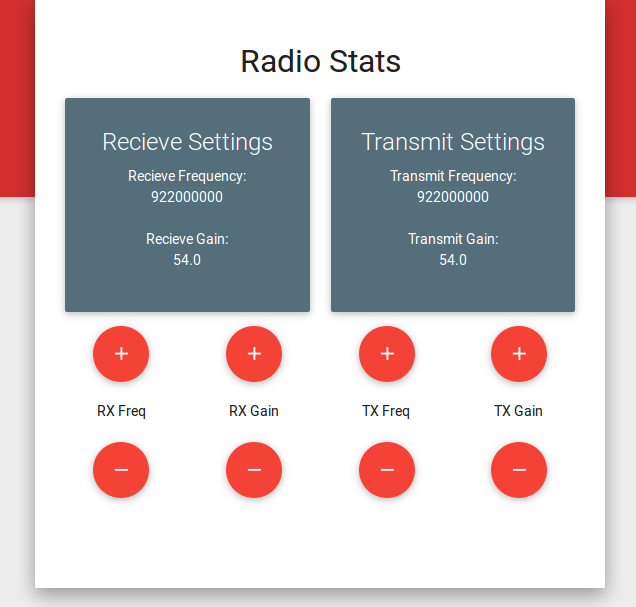
\includegraphics[scale=0.4]{WebInterFace}
	\caption{The web interface that lets the user initiate the network to hop to a new frequency. \cite{selfpaper}}
	\label{fig:WebInterface}
\end{figure}

Flask is a lightweight, open source, web framework for the Python programming language \cite{0011}. Flask was used to act as a broker between GNU Radio and any other user space applications or control systems we wished to implement. The Flask server runs the GNU Radio flowgraph in a background thread, while simultaneously configuring the TAP interface, setting up batman-adv, and starting A.L.F.R.E.D. as a background process. 

Socket.IO is a JavaScript library that enables real-time bidirectional event-based communication \cite{0012}.  SocketIO was chosen as a means of relaying data between the Flask server and other components of the system due to its speed, flexibility, and ability to broadcast messages to any connected client. Socket.IO also integrates into Flask \cite{0013} and can be used in stock Python with a client library \cite{0014}. In Flask, we create wrappers to all the necessary GNU Radio parameters so that external tools can relay data to and from GNU Radio over web sockets.  

We also use Flask to host a single webpage that displays various settings about the radio, and allows for the user to change parameters. The interface is shown in Figure \ref{fig:WebInterface}. Since our platform does not yet include logic for automatic detection of primary users, we simulate this by allowing a person to click a button to change to a new frequency. This frequency will then be sent to the Flask server using web sockets.  

\section{A.L.F.R.E.D.}

 The ``Almighty Lightweight Fact Remote Exchange Daemon," or A.L.F.R.E.D., is a system for distributing data to all nodes on a mesh network \cite{0015}. Whenever a node writes data to a channel on A.L.F.R.E.D., that data is passed between each node so that all members of the network receive the data. Typical uses for A.L.F.R.E.D. include keeping track of sensor data or building a visual map of the network. 

 An additional feature of A.L.F.R.E.D. is its ability to pass a command to the command line whenever new data is added \cite{0015}. When the transmission frequency of the USRP is changed on the Flask server, Flask sends this information along with a UTC timestamp to A.L.F.R.E.D. before changing frequencies. A small delay is created so that we can be sure the information was sent to the other nodes before the node changes its broadcast frequency.  

 When the other nodes receive the updated data table, A.L.F.R.E.D.'s callback function will run. This is a short program that parses the A.L.F.R.E.D. data table and looks for the most recent data it received. The callback function then sends the new frequency to Flask using Socket.IO which causes Flask to change the frequency in the GNU Radio flowgraph.   
%----------------------------------------------------------------------------------------

\section{Fabrication and Build Process}

The network was setup and run on a series of Lenovo S30 Computers. All computers features an Intel Xeon E5 processor and 32 GB of RAM. Each computer was running Ubuntu 14.04 LTS. The install process for GNU Radio, Batman-adv, and the rest of the technology stack is detailed in the appendix. Each computer was connected to one Ettus B200/B210 SDR using USB 3.0. 

All of the computers were connected together on a 10/100/1000 Ethernet router. This allowed for the control of the entire mesh to be handled by one computer. The popular terminal multiplexer Tmux was used in conjunction with SSH to send commands to all of the nodes in parallel. 

An additional Windows 10 laptop computer was used to control a Tektronix RSA306 wireless spectrum analyzer. This computer had an Intel i7 processor, and 8 GB of RAM. It is important to note that the RSA 306 requires a Windows machine, and therefore cannot be run on the same computer as the ones being used to run ARCAM-Net. This spectrum analyzer was used to confirm the operation of the radios and that frequency changes were occurring \cite{specan1}. 

%----------------------------------------------------------------------------------------

\section{Test Procedures}

\begin{figure}
	\centering
	\includegraphics[scale=0.4]{HopMessSmallest}
	\caption{The configuration used for the first set of tests. \cite{selfpaper}}
	\label{fig:HopMess}
\end{figure}

\begin{figure}
	\centering
	\includegraphics[scale=0.4]{NodeDrop}
	\caption{The configuration used for the second set of tests. \cite{selfpaper}}
	\label{fig:NodeDrop}
\end{figure}

In order to characterize the platform we ran three sets of tests presented below. The first test characterizes data hopping from one node to the next. The second test demonstrates batman-adv's ability to switch routes based on the quality of each node. The final tests were used to examine A.L.F.R.E.D.'s ability to be used for exchanging frequency information from node to node. 

\subsection{Network Benchmarks}

The first test was used to investigate the overhead each node adds to the network. To examine how adding hops affects the network, the USRPS were arranged so that each node was only able to directly connect to one or two neighboring nodes. This forced the nodes to need to use the multihop features of batman-adv in order to connect to the rest of the network. We used a total of 5 nodes as shown in Figure \ref{fig:HopMess}. We staggered the transmit and receive frequencies of the nodes to ensure that nodes could only talk to their immediate neighbors, forcing the network into the previously indicated configuration. The staggering of frequencies was needed to ensure each node would be unable to communicate to nodes other than its neighbors. 

 We then tested the setup at three different sets of frequencies, all within the Industrial, Scientific, and Medical (ISM) Band. We used different sets of ping tests in order to determine the number of dropped packets and the time it took to send the packets. We ran a standard ping test, one with reduced packet sizes, and one with increased time to live (TTL) settings. For a control group, two USRPs were connected together without batman-adv running. 


\subsection{Route Changes}

In a typical mesh environment, there will usually be more than one route from a source to a destination \cite{Akyildiz2009810}. In a traditional network, batman-adv switches routes based on the quality of each available link. The test was designed to determine if the same features would work in an SDRN. We initially set up four SDRs: a source, a destination, and two nodes to connect them. The first node is given a significantly larger gain in order to confirm that batman-adv will recognize that this is a more ideal path to the destination. Then, once the route is placed into the routing table, we lower the gain to 0 in order to force a transition to the other node. We then confirm that batman-adv is still able to find the new route. This setup is shown in Figure \ref{fig:NodeDrop}.



\subsection{Frequency Distribution}

In the final test, we tested to evaluate if A.L.F.R.E.D. would properly relay frequency changes over the mesh to other nodes. The user would increase or decrease the frequency using the web interface in order to simulate a cognitive radio making a decision to change to a new frequency. If A.L.F.R.E.D. was able to exchange the information properly, then the routing table would still show all connected nodes. We also used a Tektronix RSA306 Spectrum Analyzer in order to conclude that the transmission was occurring on the new frequency. If A.L.F.R.E.D. was not able to relay the information to all nodes, then some would change to the new frequency while others remain. This would be reflected in the output from the spectrum analyzer. 

%\subsection{Error (inaccuracy)}
%\subsection{Energy Use}

%----------------------------------------------------------------------------------------

%\section{Test - Network}

%\subsection{Signal Strength}
%\subsection{Range}
%\subsection{Noise}
%\subsection{Loss}
%\subsection{Error}
%\subsection{Energy Efficiency}
%\subsection{Latency}
%\subsection{Throughput}
%\subsection{Topology Effects}
%\subsection{Protocol}
%\subsection{Interference}
%\subsection{Crowding}
%\subsection{Crosstalk}

%----------------------------------------------------------------------------------------
% Chapter 4

\chapter{Findings} % Main chapter title

\label{Chapter4} % For referencing the chapter elsewhere, use \ref{Chapter1} 

%----------------------------------------------------------------------------------------

% Define some commands to keep the formatting separated from the content 
%\newcommand{\keyword}[1]{\textbf{#1}}
%\newcommand{\tabhead}[1]{\textbf{#1}}
%\newcommand{\code}[1]{\texttt{#1}}
%\newcommand{\file}[1]{\texttt{\bfseries#1}}
%\newcommand{\option}[1]{\texttt{\itshape#1}}

%----------------------------------------------------------------------------------------

\section{Results}

\subsection{Network Benchmarks}

\begin{figure}
	\centering
	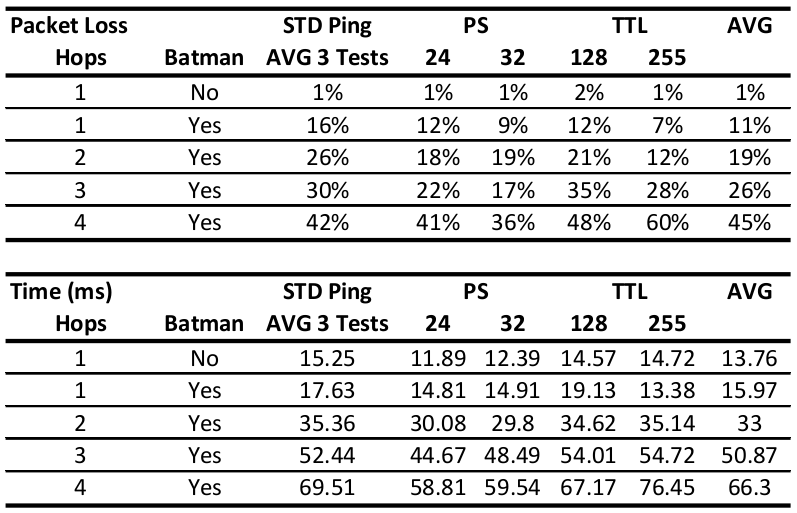
\includegraphics[scale=0.5]{902sheet}
	\caption{The data received from operating at 902/915 MHz.}
	\label{fig:902}
\end{figure}

\begin{figure}
	\centering
	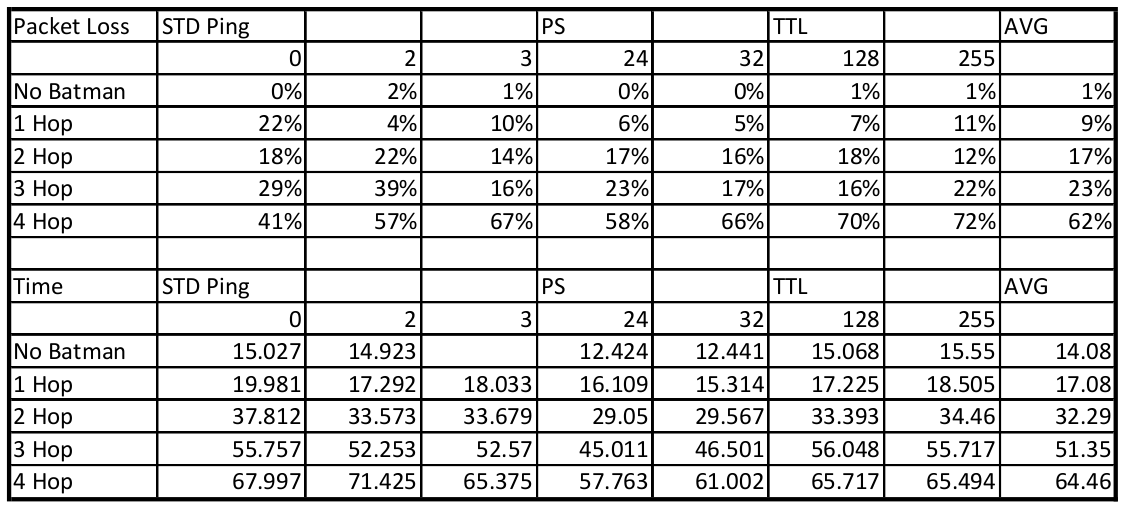
\includegraphics[scale=0.5]{2400}
	\caption{The data received from operating at 2.4/2.5 GHz.}
	\label{fig:2400}
\end{figure}

\begin{figure}
	\centering
	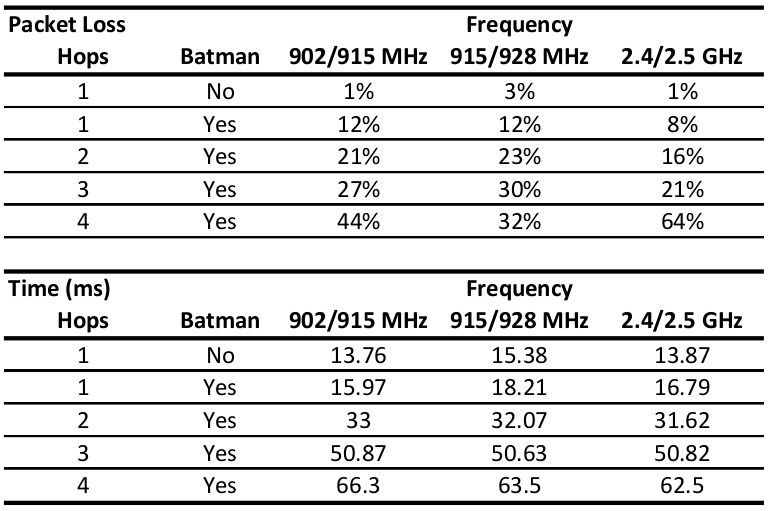
\includegraphics[scale=0.5]{alldata}
	\caption{The Averages from all three tests.}
	\label{fig:alldata}
\end{figure}

The results of the Network Benchmark tests from section 4 part A are summarized in Figure \ref{fig:alldata}. In all cases, the single point to point communication, without the batman-adv protocol running, resulted in a much lower packet loss. This served as our control group. However, in the two sets of lower frequency ratings, the packet loss remained below 50\%. Also, the increase in time as hops were added has a roughly linear change. This means the overhead of adding more hops is not unmanageable. A full listing of tests run for the 902/915 MHz, and 2.4/2.5 GHz cases are provided in Figure \ref{fig:902} and Figure \ref{fig:2400} respectively. These tables show that running at the higher frequencies causes the SDRN to drop a lot more packets, especially when moving through the full four hops.  


\subsection{Route Changes}

\begin{figure}
	\centering
	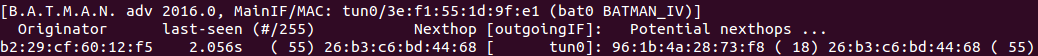
\includegraphics[scale=0.4]{2PotentialHops}
	\caption{The initial condition from the test presented in Section 4 B, where there are two possible routes the packet can take. The output is from running batctl. The link quality is listed under the column labeld (\#/255). A higher number represents a better quality connection.}
	\label{fig:2Hops}
\end{figure}

\begin{figure}
	\centering
	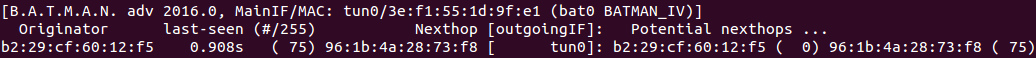
\includegraphics[scale=0.4]{hopchange}
	\caption{After the gain is reduced in the test presented in Section 4 B, the packets are now routing through a different node.}
	\label{fig:NewHop}
\end{figure}

The route changing feature of batman-adv showed success with our test setup from section 4 part B. Initially, batctl reported two possible links, one with a link quality of 55, and the other with a link quality of 18. As we decreased the gain of the intermediate node, the link quality reported by batctl also decreased. Eventually, batman-adv switched and began using the other node. At this point, it no longer saw the original node, and reported a link quality of 75 on the alternate one. The initial setup can be seen in Figure \ref{fig:2Hops}. After the change, the routing table appeared as it does in Figure \ref{fig:NewHop}. This feature works in the SDR system, and can continue to be used without significant changes.  

\subsection{Frequency Changes}

\begin{figure}
	\centering
	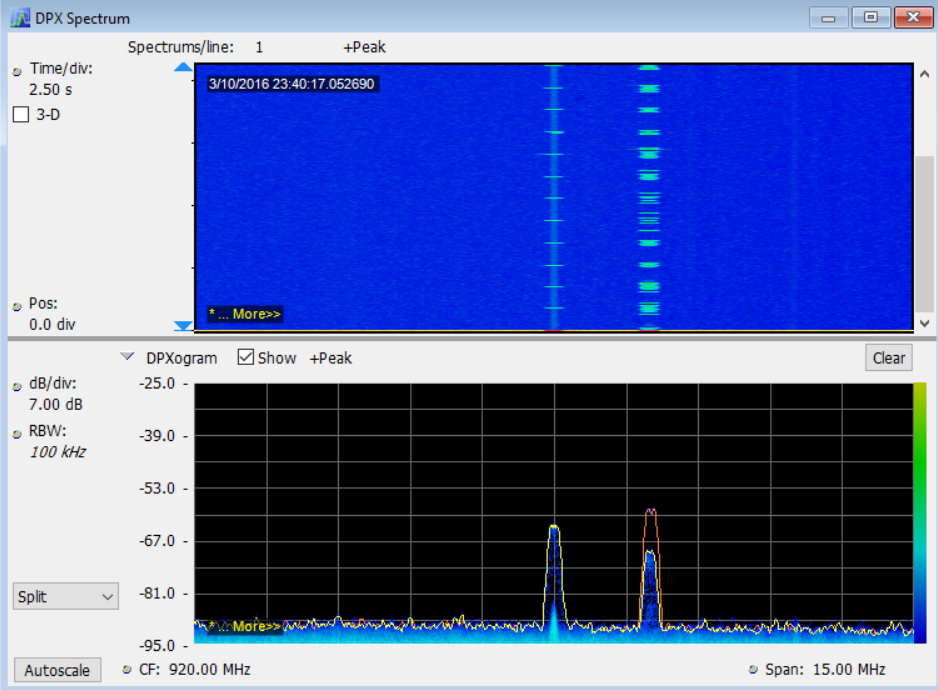
\includegraphics[scale=0.4]{FrequencyShift922-920}
	\caption{The result of using ALFRED to shift frequencies. One node is left behind as the others move to the new channel. Image collected using the Tektronix RSA306 Spectrum Analyzer}
	\label{fig:freqshift}
\end{figure}


Using A.L.F.R.E.D. to distribute frequency hopping showed mixed results. Using the setup from section 4 part C, we were able to get the nodes to change frequency in unison, but not reliably. A.L.F.R.E.D. itself is designed for a traditional Wi-Fi environment, and therefore does not have an expectation that the other nodes will become completely unreachable due to changes in operating frequency \cite{0015}. We were finding that some nodes would switch before A.L.F.R.E.D. had propagated the data table to the other nodes. This would leave one node with an out-of-date table, meaning it would not make the frequency change. In the current iteration of the project, there is no way for these orphaned nodes to find the rest of the network again. Figure \ref{fig:freqshift} shows a situation in which four out of five nodes were able to make the jump, with one node remaining at the original frequency.


%----------------------------------------------------------------------------------------

\section{Data Analysis}

In an ideal situation, we would see minimal packet loss despite introducing batman-adv and multihopping into the network. Additional tests will need to be run to discover what causes the 1 hop with batman-adv to drop many more packets than 1 hop without batman-adv. It is possible the packets are dropped as routing table information is shared, but this has not been confirmed yet. 

It is important to notice that packet loss and round trip time of packets increases lineraly with each hop. This is good, as it means each hop adds a finite amount of delay and packet loss. It would be unlikely that the delay would be constant when adding more hops, so a linear time increase is good. 

Another interesting issue with this test was that we had to stagger the operating frequencies to force the straight line topology we were looking for. Batman-adv worked very well at finding alternative paths to each node in the network. However, if the tests were left running for long periods of time it was possible the network would have been able to reconfigure into a topology other than a straight line chain. Therefore, it was necessary to manually ensure that the network would stay in the desired configuration in order to maintain a valid test. 

The route changing feature of batman-adv worked fine with the SDR hardware. Initially, there was uncertantity if batman-adv would be able to compute a proper metric for the link quality of each node. This link quality metric is what batman-adv uses to determine the best ``next hop'' to reach a different node. However, our tests showed the routing table could be properly built and updated as link quality decreased.

Our tests on A.L.F.R.E.D. showed that even though it was possible to exchange frequency information using A.L.F.R.E.D., it was not an ideal system. There was no way to ensure A.L.F.R.E.D. would pass the data to every node in the network. Therefore, the only possible way to improve upon this system would be to wait longer periods of time before shifting frequencies. If this was being used to avoid a primary user, a long delay would not be acceptable as it would interfere with the PU's use of the spectrum. Therefore, a new implementation of this feature will need to be produced. 



%----------------------------------------------------------------------------------------

\section{Assumptions and Discussion of Error}

One assumption is that the straight line configuration shown in Figure \ref{fig:HopMess} reflects how the network would behave in a full scale environment. Here we are using this configuration to determine the overhead associated with each additional hop. However, in a more robust network configuration it is likely there will be more than one path to any given node. These additional paths may be necessary to lower the overall packet loss of the network. It may be more appropriate to test this type of configuration in simulation rather than in the real world. 

We also did not test these setups in an anechoic chamber. Therefore, it is not possible to know how reflections influenced our data set. Reflections of RF waveforms can cause both constructive and destructive interference. This means that the reflections could either improve or reduce the signal quality at any given node.  

A uniform operating pattern in each node and in each antenna is assumed. Without the necessary equipment, it is impossible to truly characterize the antennas or transmission patterns of the SDRs. This is not likely to be a source of error based upon the information in the data sheets, but it is something to be aware of. 

%----------------------------------------------------------------------------------------

\section{Error Bars}

%----------------------------------------------------------------------------------------

\section{Applications}

%% Change the below if more tests are able to be run, there is probably some good quantitiative data that can be captured from SCP at least

Several application level programs were run over the network. Each application was run in both a single and multihop setting. Qualitative measurements were recorded as it was difficult to make quanititve measurements about the effectiveness of the network. The first test was run using Secure Shell (SSH). On one computer, a user would use ssh to connect to a remote computer and run a few commands to confirm operation. Next, Secure Copy (SCP) was used to transmit a file from one computer to another. A simple chat application was built in both Python and Erlang to demonstrate the ability to communicate over the network.  
% Chapter 5

\chapter{Discussion} % Main chapter title

\label{Chapter5} % For referencing the chapter elsewhere, use \ref{Chapter1} 

%----------------------------------------------------------------------------------------

% Define some commands to keep the formatting separated from the content 
%\newcommand{\keyword}[1]{\textbf{#1}}
%\newcommand{\tabhead}[1]{\textbf{#1}}
%\newcommand{\code}[1]{\texttt{#1}}
%\newcommand{\file}[1]{\texttt{\bfseries#1}}
%\newcommand{\option}[1]{\texttt{\itshape#1}}

%----------------------------------------------------------------------------------------

\section{Constraints and Limitations}



The results from our experiments show that the network is functioning as a multi hop SDRN. In addition to the experiments performed, we were also able to use Secure Shell (SSH) and Secure Copy (SCP) over multiple hops of the SDRN. However, it is clear that more work needs to be done. In a deployed network, packet loss as high as is seen in this network is not optimal. Therefore, it is important to examine ways to mitigate packet loss and increase throughput. 

For example, machine learning or artificial intelligence algorithms could be used to adjust transmission parameters as issues are detected. It is likely that a change in frequency or amplitude could mitigate some of the packet loss. For example, if the loss is due to crowding near one node, frequency hopping could be employed to shift to better operating conditions. Batctl's link quality metric, as shown in Figures \ref{fig:2Hops} and \ref{fig:NewHop} could help with finding weak nodes and making decisions. This would be the beginning of ARCAM-Net's transition from a SDRN to a Cognitive Radio Network (CRN). 

Furthermore, it would be beneficial to either improve upon A.L.F.R.E.D. or implement certain features in a new way in order to handle the frequency changing. If we have each node wait for an acknowledgment from its immediate neighbors before changing frequency, that node could then change its frequency knowing that the data will propagate to the rest of the network. 

Batctl is able to report the immediate next hop neighbors, so the program could use this information to only wait for acknowledgment from neighbors instead of waiting for the entire network to be ready to change. In order for the current A.L.F.R.E.D. setup to function, a delay was needed to give the network time to respond. Therefore, an asynchronous acknowledge would likely speed up the frequency change. 


%----------------------------------------------------------------------------------------

\section{SDR Network}

Our tests show that ARCAM-Net is a fully functioning SDR Network. We have succesfully rung ping tests, sent UDP packets, used SSH, used SCP, and even ran distributed Erlang programs over the SDRN. Thanks to the way the OSI model abstracts each layer, all programs that are designed to operate on Layer 3 or higher should see ARCAM-Net as a normal network. Though in its current state it is slower than a traditional WiFi network, there is nothing preventing any normal program from using the SDRN in the way it would use a Wi-Fi or LAN. 

%----------------------------------------------------------------------------------------

\section{Cognitive Networks}

ARCAM-Net is not a cognitive network. However, it is certainly adaptable to be used for cognitive network testing. The web interface is meant to be used as a tool for simulating cognitive events. When the user clicks a button to increase or decrease the frequency of operation, this is akin to a decision that the node itself can later make. Using SocketIO, the node can make a decision to change frequency and then send the new frequency to the Flask server. The Flask server will then update GNU Radio with the new frequency. This way, the logical decision making can be abstracted from the standard operation of the SDR. 

In our testing we determined A.L.F.R.E.D. is not a good fit for transmitting frequency data. But we can use whatever system eventually replaces A.L.F.R.E.D. as part of the cognitive network toolchain. When a node makes a decision that it wishes to change frequency, it can use this tool to distribute the information to the rest of the network. 

\section{Applications}

All of our application layer tests showed that programs could be run over the network. SSH was able to run commands from computer to computer. SCP was used to successfully send data to and from different computers over the network. The python and erlang chat applications worked succesffully and were able to transmit messages. Erlang itself is a programming language aimed at working in distributed systems and presents a unique opportunity for future work. 
 
% Chapter 6

\chapter{Conclusion} % Main chapter title

\label{Chapter6} % For referencing the chapter elsewhere, use \ref{Chapter1} 

%----------------------------------------------------------------------------------------

% Define some commands to keep the formatting separated from the content 
%\newcommand{\keyword}[1]{\textbf{#1}}
%\newcommand{\tabhead}[1]{\textbf{#1}}
%\newcommand{\code}[1]{\texttt{#1}}
%\newcommand{\file}[1]{\texttt{\bfseries#1}}
%\newcommand{\option}[1]{\texttt{\itshape#1}}

%----------------------------------------------------------------------------------------

\section{Summary}

ARCAM-Net allows for researchers to create a fully functioning SDRN in a short period of time. In it's current form, ARCAM-Net's auotmated processes could scale to up to 255 simultaneous nodes. More nodes could be added with only a few changes to the start scripts. ARCAM-Net is designed to bridge the Open-Mesh and GNU Radio projects while providing researchers with the tools they need to design, experiment, and test. 

%----------------------------------------------------------------------------------------

\section{Conclusion}

This work represents a first step in a longer term project to create a fully functioning SDRN. The work demonstrates the potential for using GNU Radio in conjunction with batman-adv and other Open-Mesh solutions. As the work continues forward, we hope the testbed can serve as a collaboration point between GNU Radio and Open-Mesh.

Both represent next generation, open source, wireless solutions and could likely benefit from collaboration between the two projects. This work can be used as an excellent starting point for anyone looking to get an SDRN up and running quickly to begin prototyping other sections of the tool chain. We plan on releasing the code as well as a handful of tools to help other researchers get started. We hope that this will serve as the first step in creating an equivalent Cognitive Radio Network platform and testbed. 

%----------------------------------------------------------------------------------------

\section{Recommendation}

The focus of this document is on ensuring that the platform is well described. ARCAM-Net should be built upon, not rebuilt again and again. The main chapters serve as a description of the project while the appendecies can be treated as a manual of operation. It is important to continue to document and project and ensure easy access to the documentation to outside parties. As with any platform, the value is in numerous groups working together on a standard set of tools. If the documentation lags behind the project, then it becomes too difficult for new users to join. 

%----------------------------------------------------------------------------------------

\section{Future Work}

There are many areas of this project that can serve as starting points for new projects. First, A.L.F.R.E.D. needs to be replaced by something more robust. A.L.F.R.E.D. could continue to be used to store distributed data that will not change often, but should not be used to store frequency data. Instead, a new tool will need to be create that can safely propagate data to other nodes, and wait for an acknolwedgement of the received information. This tool will be useful in creating the next major revision to ARCAM-Net. 

As stated previously, ARCAM-Net is a SDRN, not a CRN or CRAHN. In order to move from an SDRN to a cognitive radio environment, it will be necessary to begin to implement artifical intelligence and decision making in some form. The decision making could be split Layer 1 and Layer 3 decision making. On Layer 1, DSP would be employed to look for PU's, noise and distortion on incoming packets, overcrowded networks, and other issues. Once these problems are deteced the system will then switch to a new frequency. On Layer 3 the nodes will look for excessive dropped packets, poor batman-adv link quality, orphaned nodes, and other factors. The system will then adjust gains and frequencies until this layer has been optimized. 

While running experiments, batctl was used to monitor the quality of each node. Though batctl works fine for a few nodes, as the network scales it would make finding issues and bottle necks more difficult. Another great way to improve upon the current project would be to implement a more interactive environment for monitoring the network. A central ``control'' server could be created to monitor all of the nodes on the network and display information in a 2D or 3D environment. This would be much easier to use than batctl, as batctl produces different data on each node and therefore must be monitored on many computers simultaneously. 

\section{Applications}

%----------------------------------------------------------------------------------------


%----------------------------------------------------------------------------------------
%	THESIS CONTENT - APPENDICES
%----------------------------------------------------------------------------------------

\appendix % Cue to tell LaTeX that the following "chapters" are Appendices

% Include the appendices of the thesis as separate files from the Appendices folder
% Uncomment the lines as you write the Appendices

% Appendix A

\chapter{Running ARCAM-Net} % Main appendix title

\label{AppendixA} % For referencing this appendix elsewhere, use \ref{AppendixA}

This appendix will serve as a ``How-to'' manual for getting started with ARCAM-Net. 

\section{Configuring the Computer}

First, Ubuntu 14.04 LTS will need to be installed on each node computer. Installing Ubuntu is beyond the scope of this document. However, there are plenty of easy to follow tutorials available online. 

Once installed, the remaining steps can be done manually, or you can use a shell script I created to automate most of the process. This shell script is available \href{https://github.com/jmccormack200/GnuRadio-Vagrant-Script}{on Github}. As the name of the repository suggests, you can also use this to setup and configure a virtual machine to run the SDR software using Vagrant and Virtual Box. If you are unable to install an OS on the computers you are using, this is a good alternative. Please be aware that both options involve a lot of downloading and compiling of software. This process can take up to 8 hours so be sure to have plenty of time to let this run. An internet connection is required. 

\subsection{Installing Natively}

\code{git clone https://github.com/jmccormack200/GnuRadio-Vagrant-Script.git}
\code{cd GnuRadio-Vagrant-Script}
\code{sudo sh bootstrap.sh}


\subsection{Installing Through Vagrant}

Download and install Vagrant and Virtualbox to your computer. Then run:

\code{vagrant up}

The rest should be configured automatically.

\subsection{Manual Install}

If you prefer to do things yourself just be sure to follow along with the ``bootstrap.sh'' file below:

\lstinputlisting[language=bash,caption={Installer Shell Script}]{bootstrap.sh}

\section{Getting The Flowgraphs}

TODO once the flowgraphs are in their own repo. 

\section{Running The Flowgraphs}

TODO

\subsection{Just the Mesh Network}

\subsection{Raising the Bat Signal}

\subsection{TMux Script}

\subsection{Full Web Server}



%\chapter{Notes}

\newcommand{\shellcmd}[1]{\\\indent\indent\texttt{\footnotesize\# #1}\\}

\section{Introduction}

	The following document will contain information related to my efforts in software defined radio.
	From time to time, the document may include information on other topics as well. It will initially
	serve as a day to day journal of my activites. After a certain discovery phase, this document will
	be updated to create a manual or tutorial for future students to learn from. It is not recommended
	that the document be used for self study until a newer version is created. Many of the steps 
	that are outlined will be dead ends or poor practices while the disocvery process takes place. 
	
	Starting from the bottom and working up may be useful. 

	\newpage

	\section{7-1-2015}

	Currently working on using the RTL SDR. 

	What I have learned so far: 
		\begin{itemize}
			\item This SDR is different than a FUNCUBE dongle
			\item It will work from around 500 Hz to 1700 Hz
			\item It can only RECIEVE 
		\end{itemize}
	The fact that this can only recieve is by far the largest setback.
	This will ultimately not be what we can use for cognitive radio. 

	However, the tutorials still seem more widely available than those
	found for the BladeRF which is bi-directional. Therefore I will
	continue for a bit. It may serve a purpose as part of the larger 
	sensor network at some point. We could still use it to relay information
	over a large distance. 

	There are ``ubelite'' being sent out that are basically funcube dongle
	based satellites. These sound pretty cool. 

	I want to start taking notes in Latex so they will be more readable than
	a plain .txt file and still useable with version control. 

	I need to install texlive-full and texmaker. 

	Currently I am set back by needing to update ubuntu. I can't install
	anything else while the updates are installing. 
	
	\paragraph{Success}
		
		
	So far I have made decent progress. The RTL is working with GNU SDR. I had trouble
	at first when the kernel was loading a separate driver that bogs it down. 

	I used this command to fix that problem:
	\shellcmd{sudo rmmod dvb\_usb\_rtl28xxu rtl2823}

	There are more permanent ways of fixing the problem but I wanted to start
	with this as it is non-permanent and will default back to normal on a restart. 

	The new file in the RTL-SDR will allow you to hear FM stations. But 
	they are extremely faint. I'm going to continue to play with the file settings to
	see if I can get a clearer transmission. 
	\newpage
	\section{7-2-2015}

	I began the day with a quick interlude into learning LaTex. After about an hour
	and a half of studying I was able to produce the document you are currently reading.
	I'm not making use of many libraries but I believe it already seems more 
	organized and official than my traditional notes. Also, it is much more portable
	than a normal word document and less prone to formating failures seen in google docs. 
	
	Yesterday I got the SDR to recieve FM stations. However, they were staticy and sounded
	slowed down. I'm not sure if this is an error in my demodulation values or just that
	the computer that I'm using is too slow. I tried using a different one but that ended 
	up being slower than I remembered. I will try to get linux installed on my laptop later
	tonight when I'm done working, but I'm not confident it will work as I had trouble in the past. 

	Today I will try to replicate the results I had yesterday, but through the use of the python
	libraries instead of relying on the GNURadio GUI interface. A small note about the gui interface.
	I did learn that its possible to make variables, attach them to GUI widgets, and then alter then live. 
	It appears that having more than 3 of these can severely impact performace. To use the GUI widgets,
	simple drag one onto your workspace (I used the Wx widgets) and then give it a unique name, and 
	appropriate value range (if its a slider). Then in the blocks for different components, you can use 
	these variable names instead of hardcoded values. This is useful for gains and frequencies. 

	/paragraph{GNURadio in Python}

	I will be following the tutorial found \href{http://gnuradio.org/redmine/projects/gnuradio/wiki/TutorialsWritePythonApplications}{here}. I will begin with the dial tone generator.
	\lstset{tabsize=2, caption=dial\_tone.py,}
	%%%%%\lstinputlisting[language=Python]{../RTL-SDR/dial_tone.py}

	\paragraph{Static}
	I'm still only getting static when I run the RTL-SDR. I was able to use the GNURadio toolchain from just python
	no problem, however I still need to implent the RTL-SDR from the python toolchain. I used an additional
	tool put out by osmocom but that did not product better results. Automatic gain was on, so its possible I need 
	to manually set the gain, but I am not sure. It could also be the poor quality of the antenna. the command was:
	\shellcmd{rtl\_fm -f 96.3e6 -M wbfm -s 200000 -r 48000 - | aplay -r 48k -f S16\_LE}

	aplay is a command line utility for playing audio. I had to run that separately as piping the data did not seem to work. I got 	      this command from \href{http://sdr.osmocom.org/trac/wiki/rtl-sdr}{osmocom's website}		

	\section{07-03-2015}
	
	I will not have much time to work today due to the holiday weekend. I will try to get Linux installed on 
	my laptop in my free time. Either tomorrow or next week I will try to find a python example using the RTL-SDR
	driver. After that, I may switch gears back to the BladeRF. 
	
	\section{07-04-2015}
	Happy 4th of July! No progress will be made today as I'll be busy all day. 

	\section{07-05-2015}
	Didn't get a chance to work today either. Family event. Will continue progress tomorrow. 

	\newpage
	\section{07-06-2015}
	Back to work today. I was attempting to install a program called Gqrx. Using the instructions from their github
	I added a repository and installed just the gqrx program. However, this created a massive conflict in my repositories. I 
	uninstalled and figured I would just go back to working on the FM model to see if I could be sure its working right. However,
	installing that package messed up my installation of gnu radio. So now I must uninstall and reinstall evertyhing. At the time, I was following this tutorial \href{https://github.com/mossmann/hackrf/wiki/Installing-gnuradio-on-Ubuntu-14.04-with-the-packaging-manager}{On Gqrx}. I found a person with a similar problem to mine \href{https://github.com/kpreid/shinysdr/issues/12}{here}. 
	There are instructions below on how to reinstall everything. I will be trying that next and will hopefully get back to where
	I was. It may also be time to start learning more about virtuan environments or just how to reimage a computer quickly.	 

	Currently trying to use the following command to reset the broken packages. This is taking a long time so I will have to wait
	for it to finish in order to continue reinstalling gnuradio. The command is:\shellcmd{sudo apt-get dist-upgrade}	
	This did not end up working. Next I tried using aptitude, which as I have read, will work to fix these broken dependencies and
	packages. The command for that is: \shellcmd{sudo aptitude install <packagename>}
	Still trying to get everything installed and working. The repository made GNURadio work again, but I lost the Osmocom
	packages. Still trying. I have been following the instructions direct from osmocom but I'm getting errors related to
	``Gruel'' when I try to use cmake. 
	\paragraph{Success}
	Finally remembered that the instructables I was using previously had the commands listed (although for arch). The three
	necessary components can be installed by using:\shellcmd{sudo apt-get install gnuradio}\shellcmd{sudo apt-get install rtl-sdr}\shellcmd{sudo apt-get install gr-osmosdr}
	As a note, the instructable used arch linux and the final package was installed as gr-osmosdr-git. Debian/Fedora/Arch users
	may need to use this form of the package instead of gr-osmosdr. Another github was found \href{https://github.com/csete/gnuradio-grc-examples}{here} with plenty of examples. They may be out of date as the AM example did not compile correctly. Another useful site was \href{https://tapiovalli.wordpress.com/2014/08/02/rtl-sdr-gnu-radio-and-building-my-own-am-receiver/}{found here} this site had
	a single example, but it seemed to be working. I'm going to try to test to see if I can use my CB radio with this. I 
	think it will be too low of a frequency, but this would make testing the blade very easy as I can control the transmission
	with just the hand held radio. 
	\paragraph{R820T} So after trying to find a software solution for determining which tuner the device was using, I decided 
	that the smarter solution was to just open the SDR up. The chip inside is the Rafael Micro R820T. This is GOOD. Next to the
	elusive E4000 this is the best possible tuner to have. Its range is 24-1766 MHz. Not quite as high as the E4000 but much
	lower than that one and much higher than any other tuner that it could have had. I'm pretty happy. The device came apart with
	no tools or fuss, everything was just snapped together. The device even went back together when it was done!
	\paragraph{CB Radio} After a bit of struggling it looks like I'm able to pick up CB signals. The main issue I have now
	is that without better knowledge of signal processing I can't properly adjust the FIR filter. So I am able to recieve
	CB signals but they are not specific to any channel. The antenna that comes with this RTL-SDR is also awful. If I
	transmit over wireless I recieve really garbled sounds. If I unscrew both antennas and connect by contact it is crystal
	clear but still not on any specific channel. I don't think I'll spend much more time on this however. The file is on github
	under the name airband\_4.grc and airband\_5.grc. The 5 was an attempt to fix some of the issues with the downloaded file.
	It was called airband\_4 on the website because it was able to pickup 4 different AM broadcasts used by airplanes to
	communicate. 
	\\\\
	I found two resources to keep track of for general SDR and DSP information.
	\begin{itemize}
		\item http://complextoreal.com/tutorials/\#.VZr6nKH7s\_t
		\item http://greatscottgadgets.com/sdr/
	\end{itemize}
	
	\newpage
	\section{07-07-2015}
	Today I will be taking a look at the bladeRF SDR. The first problem that comes up is it appears I forgot to bring 
	a compatible antenna with me. I have to double check all my stuff to be sure, but due to the typically large size of
	these antennas I think it is likely that they got left behind. 
	Anyway, despite not having an antenna I'm going to push on anyway and then see what I have lying around. I should be able
	to order something on Amazon fairly quickly if needed anyway. Nuand is nice enough to have a fairly detailed set of
	documents on their github account. It also looks like these may have been updated since the last time I went through this
	process. The github account is found \href{https://github.com/nuand/bladeRF/wiki#Getting\_Started}{here}. I also just saw on
	this webpage that there is now matlab support for the bladeRF on windows. I'm not sure if this was always a feature 
	or if this is indeed new to the program. Eitherway it is something to be aware of. It has support for Simulink too. 
	
	Following the tutorial, the first step is to add the appriproate repository so we can download the files. There is a 
	snapshot section that allows you to get the most up to date releases but these are usually far from stable. The commands
	used are. 
	\subsection{Install BladeRF}
	The commands are:
	\shellcmd{sudo apt-get-repository ppa:bladerf/bladerf}
	\shellcmd{sudo apt-get update}
	\shellcmd{sudo apt-get install bladerf}

	Of course I immediately get an error saying ``you have held broken packages.'' I should probably do more research into how
	to avoid this scenario, as it seems to come up quite a lot in working with GNURadio. This could be related to using the
	other PPA from before. I'm going to try to use aptitude to install this and see if that helps. Aptitude seems to be able
	to solve the problem, however it will be removing:
	\begin{itemize}
		\item gr-osmosdr (which I know I need)
		\item libbladerf0
		\item libgnuradio-osmosdr0.0
	\end{itemize} 
	So I know that all three of these libraries are needed to run the blade and all but the libbladerf0 are needed to also
	run the RTL-SDR. I'll give it a shot and see what happens, I can always reinstall from the repository (I Hope). After running 		\shellcmd{sudo aptitude install bladerf} and accepting their suggestions it seems to have installed properly. I also ran:
	\shellcmd {sudo apt-get install libbladerf-dev} but it seemed to have already been installed. Now we can install the 
	updated FPGA drivers. 
	\subsection{Download new firmware}
	The commands are:
	\shellcmd{sudo apt-get install bladerf-firmware-fx3}
	\shellcmd{sudo apt-get install bladerf-fpga-hostedx40}
	\shellcmd{sudo apt-get install bladerf-fpga-hostedx115} 
	It's worth noting that we have the x40 not the x115 so we only need to install the x40. 
	\subsection{Reinstall GNURadio}
	The next step seems to indicate that
	I should build the gnuradio from sources and not use the version found in the repository. Luckily, BladeRF links to a 
	download script that pretty much puts cruise control on. Hopefully you have luck too. Here are the commands. 
	\shellcmd{mkdir -p ~/software/gnuradio-build}
	\shellcmd{cd ~/software/gnuradio-build}
	\shellcmd{wget http://www.sbrac.org/files/build-gnuradio}
	\shellcmd{chmod +x ./build-gnuradio}
	\shellcmd{./build-gnuradio -m prereqs gitfetch}

	It took about 15-20 minutes to finish but everything downloaded successfully. Afterwards its necessary to actually build
	the downloaded programs. I followed the steps outlined to build GNURadio and the program halts halfway through with a 
	cryptic error message. Hopefully I can diagnose the problem because it took roughly an hour to get that far.  
	 	
	\paragraph{Success!} I ended up needing to use the Pybombs tool. It worked like a charm. This is linked to in the github
	wiki mentioned above and also found on the GNUiRadio webpage.

	\newpage
	\section{07-08-15}
	Today I will be traveling and not have much time to work. I spoke too soon on the success of pybombs. It looked like it
	worked and it did install the BladeRF software properly, however the GNURadio software did not. I tried several times
	and at one point got an error about the jdk which wasn't listed as a prereq. I tried the plain build again and got much
	further (89\% vs 56\% originally). I'll try running it again and see if it goes any further. 

	\section{07-09-15}
	Today's focus switched to some open tasks I had with Dr. Integlia. The first is a comparison of various FPGA platforms
	available. After looking at everything, I am most excited by the offerings from digilent, especially the Zynq based boards.
	These have an onboard FPGA and a microprocessor onboard. I also prepared a comparison of SDR platforms. One board even 
	had a Zynq SoC on board that was programmable. This could lead to interesting research down the line as students become
	better at using the FPGAs. The FPGA comparison is available in this repository but for now the SDR is not. I will try
	to migrate it here soon too.

	\section{07-10-15}
	Today I started the Literature review. There is a lot of ground to cover. I got through 14 sources. So far the general
	gist of what I've read is that the USRP is the go to SDR for research, but that people are excited by the RTL-SDR. 
	GNU Radio seems to be very well recieved for both simulation and real world testing. I'm curious to see if some of the
	other software tools identified have a following in the academic world too. 

	I also learned how to use the IEEEtrans format for Latex and how to use Bibtex.

	\section{07-11-15}
	I won't have as much time to work today but I will try to get some amount done. I need to port the FPGA comparison
	to excel and continue the Lit Review. I will be trying to spend most of the afternoon working through Node.js and 
	research graduate schools. I've been keeping up on Node.js fairly well but have been falling behind on Grad school 
	searches. 

	\section{07-12-15}
	Today I will be converting the Latex notes into an excel spreadsheet for sharing. I may not have much time to work
	today or tomorrow but I will put full days on Tuesday and Wednesday. 

	\section{07-13-15}
	I'm going to try to make some more progress on the SDR today. I realized I may be more limited by this computer
	than I thought. It only has USB 2.0's at best and that could be throttling it too much as this is a USB3.0 boad.
	Regardless, I'll keep trying to build GNURadio for it to at least get the correct way to set that up. 

	First run: \shellcmd{git clone https://github.com/Nuand/bladeRF.git}
	
	From there I followed the directions found on their github account 
	\href{https://github.com/Nuand/bladeRF}{here}. In step four I switched to the directions
	\href{https://github.com/Nuand/bladeRF/tree/master/host}{here} and was able to build the software without errors.
	You can check to make sure it worked by running \shellcmd{bladeRF-cli -e info -e version} or
	\shellcmd{bladeRF-cli -p} So now again I was back to the point where I needed to build GNURadio. I also need to
	load the drivers to allow for the expansion board, but one step at a time. 

	Here I would like to point out that it is possible to just use a live CD to run all of this without having
	to configure anything. However, the live CD does not come with the ability to install itself. I'm not sure
	what their thought process was for that, maybe to keep everything fresh and up to date, but it is a huge inconvience. 
	If all else fails, the live CD combined with github would allow you to rebuild the environment pretty quickly each time.
	There is also direct support for bladeRF in Pentoo, a penetration testing varient of Gentoo. I can try this route if all
	else fails. 

	I am currently Running PyBombs again to try to get GNURadio to install. Hopefully it works this time, but it is
	unlikely that it will. 	
	
	\section{07-14-15}
	I don't want to speak too soon but it looks like GNURadio may have installed. I need to make a note of the following:
	\shellcmd{ \$prefix = ~/software/BladeRF/bladeRF/build/target}

	I had been running the following without the sudo command, adding sudo seemed to work. I'm not sure why I didn't see
	a clearer error before:
	\shellcmd{ sudo ./pybombs install gnuradio }
	
	For reference. Pybombs is located here:
	\shellcmd{~/software/BladeRF/bladeRF/build/pybombs}

	The steps to open GNURadio were:
	\shellcmd{:~/software/BladeRF/bladeRF/build/pybombs\$ ./pybombs env}
	\shellcmd{~/software/BladeRF/bladeRF/build/target\$ source setup\_env.sh }
	\shellcmd{~/software/BladeRF/bladeRF/build/target\$ gnuradio-companion} 

	After installing a few other modules and running an old test program, I can confirm that it is back up and running
	with the RTL-SDR. Now I am beginning the test with the BladeRF. One problem with the BladeRF is in order to easily
	test a signal I will have to use the transverter board. This is mostly because FM/CB Radio channels are below
	the normal operating range of the board. To activate the transverter board use the command:
	\shellcmd{bladerf-cli -i}
	\shellcmd{xb 200 enable 200} 
	Note the spaces in the command. The first command is just used to bring up the interactive inteface. This command was
	listed wrong on the wiki page, so I submitted a request to edit it accordingly. 

	A book to be aware of can be found 
	\href{http://people.scs.carleton.ca/~barbeau/SDRCRBook/index.shtml}{here}. This book's link was also incorrect
	so I fixed that on the wiki as well. 
	
	The biggest issue now is trying to remove the DC offset. Everytime I open the radio in the GNU Radio Companion there is a
	large spike in the center, and no audio is heard. Currently, my computer keeping freezing whenever I try to run
	anything using the BladeRF, I believe this may have to do with the limitations of this computer. I will begin trying to
	get Ubuntu running on my laptop tonight. First I have to clear off a lot of space on the harddrive. It may
	also have to do with the fact that I am using USB 2.0 ports on this computer. If thats the case, chaning to my laptop
	will not fix the problem.

	\section{07-15-15}
	Spent today trying to install Linux on my laptop. It still isnt cooperating. The problem is the laptop already has 4 
	partitions on it and HP did not make any of them extended by default as it should be with that many. I am currently
	trying to copy everything from a recovery partition, onto the main hard drive. I'll then wipe that partition and reformat
	it. Hopefully it doesn't corrupt my computer. After correspondance with Dr. Integlia, I am now aware of some other ongoing
	goals. These include:
	\begin{itemize}
	\item Preparing for next semester's courses
	\item Creating a short document
	\item Creating a longer more comprehensive document
	\item Identifying more conferences
	\end{itemize}
	I will continue spending today trying to install ubuntu and begin the transition tomorrow.

	\section{07-16-15}
	I ended up breaking my computer today while installing Ubuntu and corrupting the windows portion. I unloaded
	the documents I needed and then starting over with Windows 10 and Ubuntu. Everything works now and I can access
	google drive again.
	
	\section{07-17-15}
	Worked on the document for Harris corporation. The document can be found in this repository and on google drive.

	\section{07-18-15}
	I will not have much time to work today, and probably not much tomorrow. I should be able to make a bigger effort
	this upcoming week however. 	
	
	\section{07-19-15}
	Spent the day going over advanced MongoDB work in Node.js. I also had time to begin creating the example problems
	for the Circuits I class. I will be traveling tomorrow.

	\section{07-20-15}
	I will be traveling today with limited access to a computer until tomorrow. 

	\section{07-21-15 to 07-24-15} 
	I am traveling with limited access to SDR equipment. I have been continuing with the 
	literature review list this week and hope to have 20 sources idenfitied by Monday

	\section{07-25-15}
	Today I will be working remotely from a friend's office for a few hours. Going to try either
	getting the SDR back online or to try to finsih up the literature review. 

	\subsection{PyBombs}
	I still havent had luck with pybombs on the HP Laptop I am working from. It worked on the older computer no problem once I used sudo. I am currently reinstalling it. I have noticed that
	if I sudo whilte running PyBombs for the first time then the program is not able to be installed. The only chnanges I made this time were selecting``Force install'' for everything I knew
	I would need ahead of time, and setting the number of threads that make could use to 8. I'm not sure if this will prove to be helpful at all. The 8 threads may have been too many as now
	I'm having trouble running other programs at the same time (music slows down and skips and even vim is noticeably less responsive). 		
	\\It looks like everything is now installing correctly. The only changes were made were the ones specifed. 
	After install gnuradio, I'm not installing RTL-SDR, BladeRF, and some other packages that
	sound useful. Once they are done installing its important to remember that you actually
	need to activate them within the environment you are using. They will not stay 
	permanately active in linux. To do this we navigate to the ``source'' destination. For me,
	I just had to go one folder up, and then it was listed under target. If you cant find where
	it is, just install something else and pay attention to where it says it is writing the files
	. Then go to the appropriate folder. Once in there, run:
	\shellcmd{source setup\_env.sh}
	After testing it seems everything is back to working, at least with the RTL-SDR. Now I can
	begin testing with the BladeRF upon my return home. An important note is that I had
	a slowed down audio effect. It turned out I had miss matched sampling rates. One was being
	set manually, while another was being set by a variable. I hadn't noticed that there
	was a discrpency and now the audio sounds normal. 


	\section{07-29-15}
	I was able to do a quick test once I got home to try out the BladeRF. It is working with 
	GNU Radio now but still needs to get the DC offset fixed. 

	\section{08-04-15}
	I'm back to working on the BladeRF after a brief hiatus. Currently, I am seeing if I had to
	reload the FPGA manually. To do this I use the command:
	\shellcmd{bladeRF-cli -l <path/to/fpga/file>}
	In my case, the fpga file was stored in downloads. The FPGA file can be found on the Nuand
	website. I also learned that there are string arugments that allows GNURadio to add the xb200
	as well as automatically load the FPGA firmware. More information can be found
	\href{http://sdr.osmocom.org/trac/wiki/GrOsmoSDR}{here}. 

	\subsection{09-14-15}
	Finally back at it. Today I will be focusing on the Ettus Research USRP B200 board. I'm going to try to follow
	the tutorial found at \href{http://www.ettus.com/kb/detail/software-defined-radio-usrp-and-gnu-radio-tutorial-set}{Ettus Research}.
	I was able to use pybombs to install the first set of software. This was simply called ``UHD'' under the hardware tag in pybombs. 
	As last time, make sure you start pybombs with sudo. There was another set of drivers called ``Ettus'' that would not install. 
	I later saw this comand \shellcmd{sudo apt-get install libuhd-dev libuhd003 uhd-host}
	It said the last two were already installed, but then installed libuhd-dev. I'm still getting errors that the device is not
	found in GNURadio. Typing in ``lsusb'' shows that Linux doesnt seem to recognize the device. I'm going to reboot and see if that helps. 		

	That did not fix the issue. Next, I double checked that ``apt-get'' covered everything. As some part of the install may be from pybombs,
	which creates a virtual environment, I'm hoping that this does not cause a mismatch. Ok, so that had no effect. I'm going to google
	a bit more and see if I can figure out what I'm missing. \shellcmd{uhd\_find\_devices} Can be used to locate the device. Originally, it was 
	throwing an error message. Similar to the below: 
	\shellcmd{/usr/bin/uhd\_find\_devices: symbol lookup error:}
	\shellcmd{/usr/bin/uhd\_find\_devices: undefined symbol:}
	\shellcmd{\_ZN3uhd6device4findERKNS\_\_\_13device\_addr\_tENS0\_15device\_\_\_filter\_tE}
	Which brought me \href{http://lists.ettus.com/pipermail/usrp-users\_lists.ettus.com/2014-November/011546.html}{here}. Eventually,
	I discovered that the main issue was I had used the repositores to download the 3 files shown above (libuhd-dev, libuhd003, uhd-host) and then
	also done the commands shown below:
	\shellcmd{sudo bash -c `echo ``deb http://files.ettus.com/binaries/uhd/repo/uhd/ubuntu/`lsb\_release -cs` `lsb\_release -cs` main'' > /etc/apt/sources.list.d/ettus.list'}
	\shellcmd{sudo apt-get update}
	\shellcmd{sudo apt-get install -t `lsb\_release -cs` uhd}
	When I went back and used \shellcmd{sudo apt-get remove libuhd-dev libuhd003 uhd-host} and then ran \shellcmd{sudo uhd\_find\_devices} I got the below message
	showing that it was now registerd:

	-- Loading firmware image: /usr/share/uhd/images/usrp\_b200\_fw.hex... done
	--------------------------------------------------
	-- UHD Device 0
	--------------------------------------------------
	Device Address:
	    type: b200
	    name: 
	    serial: 3087692
	    product: B200
		
	However I'm still getting an ``Empty device address'' error in GNURadio. I did recently read that with out using USB 3.0 (my computer only has 2.0) It may
	be necessary to use either an external power adapter rated at 6 V, 3A or to use one of the 2 A to 1 B type connectors. I saw a brief document
	saying it may be an issue with not having root access, but running in a shell with root access via \shellcmd{sudo -i} did not change anything. 

	Eventually I Came across the command \shellcmd{uhd\_usrp\_probe}. This loaded the firmware and FPGA. After running this and returning to GNU Radio, I still
	am getting the errors as before. It looks like the problem may be in switching into the virtual envinronment created with pybombs. I ran the uhd\_usrp\_probe
	command again and it mentioned that there were no images installed. The error message provides a command to run which will download the images. 
	The command for me was \shellcmd{~/software/target/lib/uhd/utils/uhd\_images\_downloader.py} But make sure whatever you run is whats given to you
	in the error output. I then ran the uhd\_usrp\_probe command again but got errors about the compatibility error:
	\shellcmd{Error: RuntimeError: Expected firmware compatibility number 8.0, but got 7.0:} With information saying to run the same image downloader python
	script. 
	
	At this point I realized I messed up more than I can probably recover from easily. I tried to delete the images but wasn't double checking the folder I was
	in and removed the entire target directory that pybombs outputs to. So I'm going to cut my losses and go back to the Ettus page and install GNU 
	radio per their instructions instead of fighting pybombs to get everything to work. 
	
	While going through the documentation trying to find the GNU Radio section, I realized there is a post-download set of instructions found
	\href{http://files.ettus.com/manual/page\_build\_guide.html#post\_install\_tasks}{here}. I'm going to go through those now which include
	\shellcmd{uhd\_images\_downloader}.  

	Also changing a configuration so non-root users can access the radio:
	\shellcmd{cd <install-path>/lib/uhd/utils}
	\shellcmd{sudo cp uhd-usrp.rules /etc/udev/rules.d/}
	\shellcmd{sudo udevadm control --reload-rules}
	\shellcmd{sudo udevadm trigger}
	For my case, <install-path> was simply ``usr''. 

	I was hoping to just use apt-get to install gnuradio but that installs otherfiles not compatible with the UHD drivers installed earlier. 
	Using the same remove command we used the last time we got the error message worked (apt-get remove gnuradio was all that was really needed though). 
	Back to square one. 
	
	\section{09-15-15}

	Last night before class I ran the GNURadio build script found \href{https://gnuradio.org/redmine/projects/gnuradio/wiki/InstallingGRFromSource#Using-the-build-gnuradio-script}{here}. 
After it ran I was still having issues. I tried re-running it to just install
	the UHD Drivers, but I had to go to class. When I got back it was waiting for a user acknolowedgement (press the Y key). So I don't believe it actually ran.
	When I got in today I ran \shellcmd{sudo apt-get remove gnuradio} again to see if that would remove the build script install. It clearly stated it was removing
	something, but when I got back to the terminal and ran the USRP Probe command and then gnuradio suddenly everything was working. I'm assuming the one from
	sources never uninstalled and was actually the one that ended up running. Its likely I forgot to uninstall the one from the repositories and that that was
	the one that was causing issues. Either way, there is now ``appropriate sounding static'' on the audio from the FM block. I'll have to run further testing
	once I finish with TA stuff for the day to make sure its working. I should be able to broadcast FM and pick it up on the spectrum analyzers. I assume
	I will be unable to get FM in the VTC due to the nature of the building. I could always bring it outside to test though. 

	I am currently following this tutorial to try to get a transmitter setup:
	\href{http://wiki.opendigitalradio.org/Simple\_FM\_transmitter\_using\_gnuradio}{HERE}	

	\section{09-16-15}
	
	Today I succesfully managed to send FM radio broadcasts out of the SDR. The blocks can be found in this github repository. 
	I followed the tutorials from \href{http://files.ettus.com/tutorials/labs/Lab_1-5.pdf}{Ettus Research}. 

	\section{09-18-15}

	I found this helpful presentation from \href{http://ecewp.ece.wpi.edu/wordpress/wireless/files/2011/11/crtextbook\_ch18.pdf}{WPI}. 

	There's also the main webpage found \href{http://ecewp.ece.wpi.edu/wordpress/wireless/files/}{Here}

	They have a textbook available as well \href{http://www.qsl.net/yo4tnv/docs/Cognitive\%20Radio\%20Communications\%20and\%20Networks\%20-\%20A.\%20Wyglinski,\%20et\%20al.,\%20\%28AP,\%202010\%29\%20WW.pdf}{Here}

	I have success creating a python program that slowly ramps up the frequency it is outputting. Using my trusty Tivoli Audio PAL radio I was able to keep
	turning the dial to keep the signal in tune. The key was to put a separate thread to handle this task. I realized this when I saw that the gui function
	used a callback. This prevents the function that changes the frequency from blocking the flow of data through the other filter blocks. 
	This file is saved as FMThread.py.
	
	%\lstset{tabsize=2, caption=dial\_tone.py,}
    %    \lstinputlisting[language=Python]{../USRP_B200/FMThread.py}

	I also found this helpful website \href{http://www.cgran.org/index.html}{HERE} which organizes many of the various out-of-tree modules for GNU Radio.
	
	I am now following the install procedure for the gr-ieee802-11 block. 
	This block can be found \href{https://github.com/bastibl/gr-ieee802-11}{here}.

	The system seemed to install fine using te procedure outlined on the github page.

	\section{09-24-15}
	
	I'm going to try to take a deeper dive into some literature today, and hopefully identify some conferences/publications in the process. 
	
	first search term used is ``mesh network gnu-radio'', it returned 1 result

	Next I searched for examples of Batman-adv with GNUradio, but recieved no results over the course of several command variants.
	
	\section{09-25-15}

	I found an interesting talk from a technology evangelist from Ettus research. His website is \href{http://spench.net/drupal/}{here}. The talk
	can be found at \href{https://www.youtube.com/watch?v=ZuNOD3XWp4A}{this location}.

	He also discusses building a home made doppler system. Here is a presentation discussing this \href{http://static1.1.sqspcdn.com/static/f/679473/21303404/1355863220773/seeber-DirectionFinding.pdf?token=5JaIYIRnVDZKyXjyXksT%2B3xSZ8o%3D}{in more detail}.

	\section{10-2-15}

	Found another useful ppt from Ettus \href{https://archive.fosdem.org/2014/schedule/event/tutorial_ofdm_packet_transceivers/attachments/slides/383/export/events/attachments/tutorial_ofdm_packet_transceivers/slides/383/MartinBraun_GNURadio_OFDM.pdf}{here}.


		\section{10-23-2015}
		Today I started playing around with the Ettus Research E310. Im so excited to get to work with this
		piece of cutting edge technology. I was able to start by connecting to the device over 
		UART with the USB connector plugged into the ``console'' port. For Linux, this would probably work
		out of the box. For windows you'll need \href{www.ftdichip.com/Products/ICs/FT230X.html}{The FT230X driver from FTDI}
		We'll be using our noble terminal emulator Putty to help too. We need to get an x-server setup
		on our computer so that we can view the GNU Radio GUI. To do that we'll use XMING. This can be
		found \href{sourceforge.net/projects/xming}{on sourceforge}. Finally, we'll need to configure
		Putty properly as shown \href{wiki.utdallas.edu/wiki/display/FAQ/X11+Forwarding+using+Xming+and+PuTTY}{here}. 
		This let me acces GNU radio fine and I could see the window on my computer. If any of the links
		are dead, just try googling some of the keywords. Nearly all of the links I used were just
		the first or second result. 

	\section{11-1-15}
	I have started researching TUN and TAP Adapters. These seem to be the key to what we are trying to do but I am not confident enough to say that. TUNs are virtual ports that
	accept IP packets and TAPs are ports that accept virtual ethernet packets. In theory I should be able to use a TAP to abstract out the MAC Address, but that doesnt seem the case. 
	The way I understand it TAPs are the layer that connects PHY To MAC and TUNS connect MAC to layer 3. I'll continue to research these topics.

	\section{11-3-15}
	I found this link: http://www.wu.ece.ufl.edu/projects/wirelessVideo/project/GNU\_Radio\_USRP/
	Example 3 provides some insight showing that my thought process is correct. I wish there was a flow graph for reference but it is just a python file. I will continue looking into
	this.

	\section{11-7-15}
	Need to look into how the Zigbee protocol is implemented. Basically it looks like the PHY layer needs to not only accept and transmist the complex
	signal, but also needs to convert complex to and from packets. These packets may then be able to be passed to Batman adv over a TUN interface. 
	
	\begin{itemize}
	\item ask questions first posted to him directly
	\item post questions to github. 
	\item ask for 802.11 traditional transciever
	\item run zigbee
	\item run 802.11p
	\item compare the implementations and look for differences
	\item identify questions about the differences. 
	\end{itemize}

	Now trying to connect my linux laptop to the E310 using ssh -X root@192.168.1.100
	
	\section{11-14-15}
	Spent most of the day trying to build the UHD driver on the E310 itself. This took about four hours to do. There still seemed to be an issue.
	I'm going to continue orking tomorrow. The website I am looking at right now can be found here:

	\href{https://sdradventure.wordpress.com/2015/01/}{Link to the other person's website}

	\section{11-15-15}
	This E310 is still giving me a ton of problems. I spent about 3 hours this
	morning trying to get everything to place nice. The issue seems to be that
	the E310 is running UHD version  3.08 and my PC is running 3.10. I'm not
	sure how this is happening is both should have been built from sources
	which makes me think I'm either missing something in the install process
	or I have a version installed from a different source and I'm not noticing.
	When I make uninstall on both the PC and E310 there are still versions
	of the \_uhd\_usrp\_probe software. I found this message on the
	\href{http://lists.ettus.com/pipermail/usrp-users_lists.ettus.com/2015-April/013716.html}{gnuradio mailing list} that seemed to indicate I would have to roll
	back the PC version or reflash the SD card. I'll have to continue working
	for now as its going to be awhile until the B200 gets here. I may
	also continue looking into Vagrant tonight as it would be helpful
	for trying to switch back and forth between versions quickly. 


	\section{11-17-15}
	So currently it appears that I have rolled back the PC to the proper
	version of UHD and it apears this may be simple to switch between the two
	versions should I have broken something. Basically, the repository version
	of UHD is version 3.008 and the sources version is 3.010. So a 
	make install or make uninstall will add and remove 3.010. On the other
	hand a sudo apt-get install uhd or sudo apt-get remove will do the 
	same for version 3.008. Hopefully when I try this tonight everything works
	out. This will also help when it comes time to fix the vagrant file.
	
	Currently with vagrant I am unable to install UHD from the gnu radio
	sources. If we end up going with 3.008 I will just apt-get UHD. When I 
	run GNU-Radio companion I get an error about the python path. If this
	goes away I wont discuss it further, but if it continues I'll include
	some screenshots and such to help with debugging. 

	\section{11-19-15}
	This link may help clarify some issues: 
	\href{https://lists.gnu.org/archive/html/discuss-gnuradio/2015-08/msg00459.html}{Here}

	\section{11-20-15}
	Found a link to a washington state course. It has details about several lab exercises done out in both
	matlab and gnuradio \href{http://courses.washington.edu/ee420/assignments.html}{HERE}

	\section{11-22-15}
	Almost forgot to save this webtie:
	\href{http://aaronscher.com/GNU\_Radio\_Companion\_Collection/Packet\_encode\_decode.html}{Here}
	It has a lot of useful information. I was able to use it to transmit an image through a flow graph, but so far I have been unabe
	to transmit over the air. 

	Some more useful links are below:
	\href{http://www.trondeau.com/grcon15-presentations/}{Here}
	\href{http://static1.1.sqspcdn.com/static/f/679473/23657925/1381271009800/grcon13\_malsbury\_phy\_mac\_primer.pdf?token=lfzQT7OcTknN\%2F6iH3YbnHjePsug\%3D}{Here}


	\section{12-22-15}

	Finally got back to work on this after a mountain of finals and TA work. We have the B210 and I wanted to get a feel for working with the dual channels. The key is in the 
	subboards sections. RF Block A needs to be set as A:A, and RF Block B needs to be set as A:B. I was successfully able to transmit and recieve on the TX/RX line of both
	sides. 

	\section{12-23-15}

	Ran some more tests today. I was unable to get batman-adv working over zigbee following ``the easy way'' I had initially hoped. However, there are a LOT of variables and different settings that I have to confirm are all in sync before continuing on. I also am working off of just the TX/RX antennas and I am unsure if they automatically function in full duplex mode or if that needs to be managed. I ordered two additional antennas on amazon so that I can use separate TX and RX channels instead of one single channel for each. 

	\section{12-29-15}
	Met with Mathworks yesterday to discuss options from available for working with SDR. I'm excited to begin working with Houman and the rest of the team on this part of the project. Hopefully things will go smoother using a full featured piece of software versus the open source software we have been using. I would like to continue working with GNURadio while I still have a chance however as I believe some things, such as interfacing into Unity, will be significantly easier being able to use python than having to use MATLAB. 

	\section{1-5-16}

	I was finally able to test out my shell script that creates a GNU Radio Companion environment on a computer. It worked awesome but I forgot to design it to install the UHD drivers for GNURadio. I think I'll add a module that goes to the end and then downloads and opens PyBombs to allow for the rest of the modules to be installed as needed. This will make the system more robust to future changes to GNU Radio. 

	\section{1-7-16}

	Found an interesting article today: http://www.schooner.wail.wisc.edu/tutorial/docwrapper.php3?docname=gnuradio.html

	http://gnuradio.org/data/grcon11/02-ge-gr\_network\_layer.pdf

	http://www.profheath.org/research/mimo-system-prototyping/hydra-mimo-ad-hoc-network-phase-2/

	http://gnuradio.org/redmine/projects/gnuradio/repository/revisions/58bd4ceaee4884652a682297a49957137cafa56d/entry/gnuradio-examples/python/digital/tunnel.py

	\section{1-11-15}

	Found this video:

	https://www.youtube.com/watch?v=g3-SjnES0K8

	He shows a demonstration of the tunnel.py program located in gr-digital -> examples -> ofdm ->tunnel.py

	I tried this out but was unncessful in pinging. It may have to do with configuring the gateway/iptables.

	The docs say tunnel.py is a poor choice for projects and will be deprecated in favor of gr-mac.

	After rewatching the video the commands he runs are:
\shellcmd{./tunnel.py -f 910.0M -r 100k}
	\shellcmd{ifconfig gr0 192.168.200.1}
	\shellcmd{route add -net 10.10.10.0/24 gw 192.168.200.2}
	
	http://static1.1.sqspcdn.com/static/f/679473/25468067/1411397041210/Sep15\_06\_Malsbury\_Applications.pdf?token=G00WxKmbuG1znO9yu%2F2YZIQvVzg%3D

	\section{1-12-16}

	So as far as I can tell it looks like the tunnel.py file is deprecated and sore spot as far as GNU Radio's community is concerned. I'm currently looking into gr-mac and pre-cog. Its unclear which of the two is currently the well supported file (if either). There is a video explaining how to use pre-cog below:

		https://www.youtube.com/watch?v=f8emQ-TvD90

	\subsection{SUCCESS}

	Batman-adv was attached to two USRPs running on separate computers utilizing the gr-mac library fork made by Baliant Seeber. The fork can be found below:
	\href{https://github.com/balint256/gr-mac.git}{Link to Github Repo}

	This will need to be setup on two different computers using the following process:
	\shellcmd{git clone htt[s://github.com/balin256/gr-mac.git}
	\shellcmd{cd gr-mac}
	\shellcmd{mkdir build}
	\shellcmd{cd build}
	\shellcmd{cmake ..}
	\shellcmd{sudo make}
	\shellcmd{sudo make install}
	\shellcmd{sudo ldconfig}

	Balint's fork doesn't have a very good readme as of the time of this writing, but following the original jmalsbury repo the next steps are below. His fork can be found
	\href{https://github.com/jmalsbury/gr-mac}{here}
	\shellcmd{cd ..}
	\shellcmd{cd example} 
	\shellcmd{sudo gnuradio-companion gmsk\_radio.grc}
	Then Build and Run this flow chart. Then:
	\shellcmd{sudo gnuradio-companion ofdm\_radio.grc}
	Then Build and Run that flow char. Next:
	\shellcmd{sudo gnuradio-companion simple\_trx.grc}
	
	Now we need to go to the first computer and follow the below commands:
	\shellcmd{sudo python simple\_trx.py --port 12345 --radio-addr 85 --dest-addr 86}
	In a 2nd terminal type 
	\shellcmd{sudo ifconfig tun0 192.168.200.1}

	Then we will go to the other computer and run the following commands:
	\shellcmd{sudo python simple\_trx.py --port 12346 --radio-addr 86 --dest-addr 85}
	Again in a 2nd terminal type
	\shellcmd{sudo ifconfig tun0 192.168.200.2}

	Back to computer 1, in the second terminal type:
	\shellcmd{nc 192.168.200.2 12346}

	In computer 2, in the second terminal type:
	\shellcmd{nc 192.168.200.1 12345}

	you should now be able to type messages and see them appear on the other radio, if not, check all your connections and ensure there are antennas. 

	Now to add batman-adv we will go back to the first computer:
	\shellcmd{sudo modprobe batman-adv}
	\shellcmd{sudo ip link set mtu 1532 dev tun0}
	\shellcmd{sudo batctl if add tun0}
	\shellcmd{sudo ip link set up dev tun0}

	On the other computer, the same commands are issued, repeated in case they need to be changed later:
	\shellcmd{sudo modprobe batman-adv}
	\shellcmd{sudo ip link set mtu 1532 dev tun0}
	\shellcmd{sudo batctlif add tun0}
	\shellcmd{sudo ip link set up dev tun0}

	Then if you run the below command on either computer you should see one other batman node active:
	\shellcmd{sudo batctl o}

	\section{01-15-16}
		
	Confirmed that the flowgraph we are working from only uses the TX/RX antenna. This will obviously slow down the transmission of packets but may also present opportunities for using
	the RX antenna for another use such as ambient energy detection or to scan for other active channels. 

	We could potentially have this scan the ISM band and if a primary user or other instance tells the radio to move off it could then wait for a signal from another node to tell it
	which channel to begin transmitting on. 
	
	\section{01-22-16}

	Having trouble setting everything up on the new computers. Looks like the issue may be as simple as the distance between the transmitters is too far. These Antennas arent exactly great and I
	have to use the adapters with them so this is very possible. I'm going to keep working to confirm this. It still works on the first two we used so if anything I will just make an image and copy
	that to the new computers.

	\section{01-23-16}

	Ok so here is the state of affairs. We have successfully send batman-adv packets over SDR, as was noted before. However, after changing things to be ``broadcast'' under dest-addr in the virtual 
	encoder and virtual decoder I was able to successfully ping bidirectionally through 3 devices with no problems whatsoever. We are currently seeing extreme range limiting issues for some reasons
	that are currently unclear to me. I tried adjusting the frequencies through the init part of the automatically generated python scripts but that does not seem to be working. I'm not 100%
	sure why but would guess it has something to do with the fact that these files are automatically generated and are not created by a true programmer. I also think this may be the reason why
	we were having issues with the three new computers in the center of the lab. I'm hoping to run more tests before I go home today. Joe is currently running bat-vis to show me how to map topologies.

	I will need to make a quick start guide or something soon for automating the process of setuping up each node. We are planning to expand to 16 nodes and this could become quite difficult.
	I believe learning one of the terminal multiplexers such as screen or tmux would be beneficial for the future.

	Important progress/updates this morning:

	1. The board I thought was broken was just an error, I was using a USB 2.0 cable not a 3.0 cable which meant it couldn't get enough board power to broadcast, but could get enough to turn on which explains the weird error. 
	2. So far it appears the 3 computers weren't working because the boards were too far apart from one another. I realized in the original setup they were under 1 ft from one another. This is probably an issue with transmit frequency as it was operating at 980 MHz and the antennas are rated for 2.5 GHz. I will run some more tests throughout the day to confirm.
	3. I was able to successfully send packets between 3 radios today. I made three changes and now will figure out which of the changes mattered. The first change was that I noticed you could replace ``dest-addr'' (Destination address) with broadcast in the gnuradio blocks in question (virtual-channel-encoder/decoder). I also noticed that in the ``Channel Multiplexer'' it is possible to increase the ``Channel count'' number higher and it will allow for more outputs. I snaked these outputs to the same locations as the originals and this allowed for the transmission. Finally, I ensured all the boards were within a few inches of one another. I realized in the original setup we were seeing the middle board able to talk to the 2 edge boards, so wasn't sure if it was a proximity problem. Regardless, one of these should allow up to continue forward.

	If I can't get the 3 new computers working by around 4-5 today, I will work with Pat/Cody tonight to image them off of the first computer. 

	\section{01-26-16}

	Successfully switched frequencies around and managed to continue transmitting packets. I have generated two new radio flow graphs that may eventually get merged into one. The first is called:
``BroadcastMAC.grc''. This allows for the changing of TX/RX freq and gain. This also has the virtual 
channel encoder/decoder set to broadcast. I believe this needs to be running on at least one of the
radios in the mesh to work. The second block has a much larger name unfortunately and is called:
``nonbroadcastwithGreqAndMac.grc''. The difference between this and the other block is that I did not
change the virtual encoder/decoder to broadcast mode and added the additon of a spot to change
the mac address on the fly. This is useful in cases where you forget to change the mac address
before running. 

Next steps are to try to see if we can bridge internet access over these usrps with batman, to see
how batman reacts to the changing frequencies, and to take steps to allow for automation. 

As always, a more indepth literature review will need to continue. 
	
	\section{01-27-16}

	So after playing around with GNU Radio for a few hours I found a block called ``selector'' 
	within the gr-misc category. This is essentially a multiplexer that can map n inputs to 
	m outputs. A simple change of variables decides which input and which output are active. 
	This should help us with our search for PHY layer changes we had discussed. 

	Unfortunately selector only works on streaming blocks so a different device will need to be 
	created. I'm currently guessing I can make this work fairly simply by just mashing the OFDM
	and GMSK together.

	\section{01-28-16}

	Still trying to get the selector stuff to work, so far it just keeps crashing whenever I change
	sources. Here's an interesting side project that may be worth looking into at a later point in
	time: \href{https://github.com/pothosware/gnuradio/wiki}{Follow the link}


	\section{02-05-16}

	Today I finalized some target conferences and journals. The shortest deadline I can see
	is March 1st. A tight window but we may be able to push the gnu-radio/batman combination
	paper through assuming we can collect and process the data in time. The biggest hurtle will
	be getting everything done prior to spring break as I dont think I'll have much
	time to work over that week. 

	Today I will go through the Practical Evaluation of BATMAN Advanced paper with Pat to try to
	understand their test process so we can replicate some of their work with our environment. 
	This should help speed up the test development phase. I would LOVE to have all
	testing down by friday of next week so we can spend the next week drafting and finishing up
	the paper but I don't think that will be feasible as we probably need more than the 4 nodes
	we currently have. 

	\subsection{Test Plan Alpha}

	This is the initial draft of how we are hoping to test the system:
	\begin{itemize}
		\item The test plan we are basing this from mentions testing from one floor to
			another. I'm not sure this will be feasible as the layout of the school is
			not conducive to this. We will most likely have two-three setups
			where we can utilize the VTC Alone, and then several rooms
			adjacent. I like the floor plan included in their paper and would
			like to replicate that to show how the networks form. This is based
			on us being able to get more distance then we are currently seeing from
			the USRP Radios. 
		\item Radio Conditions: Here we will profile the radio with and without Batman-adv
			running to measure the RSS using a tektronix spectrum analyzer. We can
			get distance measurements to quantitatively measure the RSS level when
			we lose the radio connectivity. 
		\item Reachability and Packet Loss: From here we will ping from one node to
			all the other nodes and measure how many packets are dropped. We
			can set a number of ``n'' pings and count how many packets were dropped.
		\item Delay: Here we will use a test with ``n'' pings, but this time will measure the
			response time and find an average/std deviation to determine how slow the
			network is. 
		\item Throughput: We will have to find a tool for properly measuring a throughput
			test. We could set one node up as a gateway and use a traditional internet
			speed test but I belive that would be creating unecessary overhead. 
		\item Route Changes and Convergence: The paper is a little sparse on the description
			of how they benchmarked this. It looks like we would turn a node off and
			view how the network reacts, possibly one in the center.
		\item Frequency Based changes: I think it would be good to run all of these tests
			at several frequencies and examine the changes. This will obviously
			be dependent on the antenna used so we may need to either use
			a small band, mention this limiting factor, or switch antennas. I
			believe our antennas are also rated at 5 GHz but would have to check.
		\item Joe mentioned Using Alfred to make many of these graphs and I believe it would
			help strengthen the paper and provide useful visual aids.
		\item Link Decays: Possibly another way to organize the information and run a test
			would be to link more and more nodes and measure how the network
			degrades as more hops are added. We could measure up to 4 hops right now,
			and hopefully 7 once we recieve the next 3 radios. We could then
			test this at 3-4 frequency levels and view the results. 
		\item Frequency Hopping: We still do not have an AI based frequency hopping algorithm
			in place. I'm not confident in my ability to have one in place by March 1st
			but can do my best. It may be better to write a first draft of the paper
			not involving frequency hopping and then re-evaluate closer to the deadline.
			We can then hope to have this in place for the next two papers

	\end{itemize}

	\section{2-8-16}

	Still havent got to the testing phase. So much to do,so little time before the paper deadline. Anyway, finished the webhook stuff. Tried to see if we could
	use two channels on the B210 as part of the network, but the initial test was not promising. It said ``node alive'' for both nodes, but was filled with ``D''s which
	usually means theres errors in the stream and I wasn completely unable to ping back and forth. 
	\section{2-10-16}

	Met with Brad yesterday to discuss everything in depth. I created a new shell script called 
	raidseBatSignal.sh that should set up the batman-adv stuff automatically.
	\section{2-11-16} 

	Meeting with Matlab today. Looks like Alfred is going to help us quickly
	develop the functionality we are looking for.

	\section{2-13-16}

	Still can't figure out how to configure Alfred. It looks like parts of it are built into 
	batctl but we really need to figure out how to distribute the frequency information"

	\section{2-18-16}

	Alfred -c works, but will only run if the data was changed by someone other than the host.
	Essentially, the computer that updates Alfred will NOT have the command listed on Alfred -c
	run. 

	Additionally, the webinterface flowgraph is still running the older version. We need to update
	it to a broadcast flow graph. It is currently at a much older nonbroadcast flowgraph. 

	Furthermore, we need to create a better system for adjusting the MAC address on each node. 
	The current system will be unusable once we want to work with more than 2 nodes and is annoying even
	then. 

	Tomorrow I need to go over how to set everything up with Joe, and possibly create a written testplan
	so that he can help with that the next week/this weekend. 

	START WRITING.

	RESTRUCTURE Trello to be useable by others. 

	\subsection{ESPEAK}

	Espeak is hilarious 

	\section{2-20-16}

	After struggling for awhile trying to figure out what was going on it turned out that I did not
	actually have a functioning flowgraph until today. The problem was that though GNU Radio
	is happy to work in a thread, the GUI is not. I'm not sure why I didnt think of this before
	as Unity3D should have taught me that visuals and threads don't get along. 

	Anyway, now im going to keep working on adding the Alfred implementation. Hopefully
	tomorrow Brad will be in and I can work on the Fedora builds while he is helping to clean 
	up the rest of this code. I'm still not against abandoning flask in favor of a MQ system
	which with the right MQ system may make for a more robust system. But, with the deadline
	approaching I'm not 100 percent sure I want to start porting to a new platform. 
	\section{2-22-16}

	\subsection{batctl source build}

	We are trying to upgrade batctl and will track the needed changes here:

	\begin{itemize}
		\item{sudo apt-get install libnl-3-dev}
	\end{itemize}



	Trying to test today. Still having trouble. We can see from nodes to their next hops but not beyond that. 

	Will continue to test and report back here as we learn more

	\section{2-23-16}

	Today we are going to continue testing. To begin, we are building batman-adv 2016.0 from sources. 
	The file can be downloaded from batman's website and is installed by:
	\shellcmd{sudo make}
	\shellcmd{sudo make install}
	\shellcmd{sudo depmod -a}
	\shellcmd{modprobe batman-adv}

	\section{3-7-16}

	Helpful website for changing the hostnames of computerS:

	\url{hostnames}{http://askubuntu.com/questions/9540/how-do-i-change-the-computer-name}
	
	\section{3-28-2016}
	
	\href{http://courses.washington.edu/ee420/assignments.html}{Link To Tutorials}

	There is also a paper discussing the use of GNU Radio as a means of spectrum sensing. It is
	an IEEE paper titled "Experimental Spectrum Sensing Measurements using USRP Software Radio
	Platform and GNU-Radio." However, no code is provided, just psudocode/equations. 

	 However, no code is provided, just psudocode/equations. 
 
 	Another github to be aware of for spectrum sensing can be found \href{https://github.com/m0mik/scanoo}{here}


%\include{Appendices/AppendixC}

%----------------------------------------------------------------------------------------
%	BIBLIOGRAPHY
%----------------------------------------------------------------------------------------

\printbibliography[heading=bibintoc]

%----------------------------------------------------------------------------------------

\end{document}  
